% ============================================================
% Chapter 17 --- Submanifolds, tangent and normal spaces
% Originally: content/week-07.tex, \section{Submanifolds} (with the regular value and local
%             parametrization theorems) and \section{Tangent and normal spaces}
%             (Corsin Week 7), plus problem 7.6 from sheet 7.
% ============================================================
\chapter{Submanifolds, Tangent and Normal Spaces}
\label{ch:submanifolds}

% Transition: Claude Opus 5 (Medium)
The implicit function theorem said that a level set is locally a graph. This chapter takes that
as a definition: a submanifold of $\mathbb{R}^n$ is a set that looks, near each of its points,
like a piece of $\mathbb{R}^k$. Three descriptions turn out to be equivalent --- as a level set of
a submersion, as a local graph, and as a local parametrization --- and each is the convenient one
for a different purpose. The chapter closes with the linear algebra attached to each point: the
tangent space of directions along the submanifold, and the normal space orthogonal to it.

% Originally: content/week-07.tex, \section{Submanifolds} (Corsin Week 7)

% Source: Corsin Nick/Class Notes/Week 7.pdf, p. 2
\section{Submanifolds}
\label{sec:submanifolds}

Recall that a \newterm{$C^k$-diffeomorphism} (\cref{thm:inverse_function_theorem}) is a $C^k$
bijective function whose inverse is also $C^k$.

\begin{definition}[Submanifold]
\label{def:submanifold}
$M^m \subseteq \mathbb{R}^n$ is a $C^k$, $m$-dimensional \newterm{submanifold}
\germanfor{Untermannigfaltigkeit} of $\mathbb{R}^n$ if for any point $p \in M$ there are an
open neighbourhood $U \subseteq \mathbb{R}^n$ of $p$, an open neighbourhood $V \subseteq
\mathbb{R}^n$ of $0$, and a $C^k$-diffeomorphism $\Phi : U \to V$ with $\Phi(p) = 0$ (a
\newterm{submanifold chart}) such that
\[\Phi(U \cap M) = (\mathbb{R}^m\times\{0\}) \cap V = \{x \in V : x_{m+1}=\dots=x_n=0\}.\]
\end{definition}

% Sonnet 5 (Medium) --- FIG-W07-01
\begin{center}
\begin{tikzpicture}[>=Latex, scale=1.0]
  % Left panel: the curved submanifold M with a chart neighbourhood U around p
  \begin{scope}[shift={(0,0)}]
    \draw[blue!70!black, thick] plot[smooth] coordinates
      {(-1.6,-0.4) (-0.9,0.5) (0.0,0.1) (0.9,0.7) (1.7,-0.1)};
    \node[blue!70!black, font=\small] at (1.9,-0.4) {$M$};
    \draw[orange!90!black, thick, dashed] (0.0,0.35) ellipse (0.85 and 0.75);
    \node[orange!90!black, font=\small] at (0.0,1.25) {$U$};
    \fill (0.0,0.1) circle (1.5pt) node[below, font=\small] {$p$};
    \node[below, font=\small] at (0,-1.3) {$\mathbb{R}^n$};
  \end{scope}

  \draw[->, thick] (2.5,0) -- (3.7,0) node[midway, above, font=\small] {$\Phi$};

  % Right panel: the flattened image, R^m x {0} as a horizontal line inside V
  \begin{scope}[shift={(4.4,0)}]
    \draw[orange!90!black, thick] (-1.1,-0.9) rectangle (1.9,1.1);
    \node[orange!90!black, font=\small] at (0.4,1.35) {$V$};
    \draw[green!60!black, thick, ->] (-1.05,0) -- (1.85,0)
      node[right, font=\scriptsize] {$\mathbb{R}^m\times\{0\}$};
    \fill (0,0) circle (1.5pt) node[below, font=\small] {$0 = \Phi(p)$};
    \node[below, font=\small] at (0.4,-1.3) {$\mathbb{R}^n$};
  \end{scope}
\end{tikzpicture}
\end{center}

% Corsin's own observation; the note it used to sit in was an ainote until 2026-08-09, but by
% Test 1 in style.md it is mathematics rather than commentary about the transcription.
\begin{remark}[Why the definition is almost never used directly]
Producing such a $\Phi$ by hand is difficult even for simple $M$, so the definition is rarely
what one works with. Two equivalent descriptions do the job instead, the \textbf{implicit} one
(the regular value theorem below) and the \textbf{explicit or graphical} one (the local
parametrization theorem below). \Cref{rem:three_submanifold_descriptions} compares all three
once both are available.
\end{remark}

\subsection{The regular value theorem}

\begin{theorem}[Regular value theorem]
\label{thm:regular_value_theorem}
Suppose $U \subseteq \mathbb{R}^n$ is open, $F \in C^k(U,\mathbb{R}^\ell)$, and $y \in F(U)$. If
\[DF_x : \mathbb{R}^n \to \mathbb{R}^\ell\]
is surjective (i.e., $\Jac F(x)$ has full rank) for all $x \in F^{-1}\{y\} = \{\bar x \in U :
F(\bar x) = y\}$, then $F^{-1}\{y\}$ is a $C^k$ submanifold of dimension $n-\ell$.
\end{theorem}

% Sonnet 5 (Medium)
\begin{importantremark}[Full rank means two opposite things]
\label{rem:full_rank_two_meanings}
\qt{Full rank} is decided by the \textbf{shape} of the matrix, and the two representations of a
submanifold sit on opposite sides of it:
\begin{itemize}
  \item An \textbf{implicit} description $F : \mathbb{R}^n \to \mathbb{R}^\ell$ cuts $M$ out by
    $\ell$ equations, so $\Jac F$ is \textbf{wide} ($\ell \times n$ with $\ell \leq n$). Full
    rank $=\ell$ means $DF_x$ is \textbf{surjective}, so the $\ell$ constraints are independent,
    each one genuinely cutting a dimension. Here $\dim M = n - \ell$.
  \item A \textbf{parametrization} $f : \mathbb{R}^m \to \mathbb{R}^n$ sweeps $M$ out by $m$
    parameters, so $\Jac f$ is \textbf{tall} ($n \times m$ with $m \leq n$). Full rank $=m$
    means $Df_x$ is \textbf{injective}, so the $m$ parameters move in independent directions,
    none of them wasted. Here $\dim M = m$.
\end{itemize}
Same phrase, opposite condition. A wide matrix is never injective and a tall one is never
surjective, so there is no ambiguity in practice. But it is worth checking which side you are on
before writing down what \qt{full rank} is supposed to give you.
\end{importantremark}

% Source: Corsin Nick/Class Notes/Week 7.pdf, p. 2
\begin{example}[Circle of radius $R$]
Let $F : \mathbb{R}^2 \to \mathbb{R}$, $(x,y) \mapsto x^2+y^2$. Then
\[\Jac F(x,y) = (2x,\ 2y)\]
has full rank at every $(x,y) \in \mathbb{R}^2\setminus\{0\}$. Here $\ell = 1$, so by
\cref{rem:full_rank_two_meanings} full rank means that $DF_{(x,y)} : \mathbb{R}^2 \to \mathbb{R}$
is \textbf{surjective}, which for a single row is simply the requirement that $(2x,2y)$ be
nonzero. For $R>0$, $(0,0) \notin F^{-1}\{R^2\}$, so
\[F^{-1}\{R^2\} = \{(x,y) \in \mathbb{R}^2 : x^2+y^2=R^2\}\]
is a submanifold of dimension $2-1=1$ by \cref{thm:regular_value_theorem}. Similarly,
$\{x \in \mathbb{R}^n : |x|^2=R^2\}$ is a submanifold of dimension $n-1$ for $n \geq 1$ (the
\newterm{$n$-sphere} of radius $R$).
\end{example}

% Sonnet 5 (Medium) --- FIG-W07-02
\begin{center}
\begin{tikzpicture}[>=Latex, scale=1.1]
  \draw[->] (-1.7,0) -- (1.7,0) node[right, font=\small] {$x$};
  \draw[->] (0,-1.7) -- (0,1.7) node[above, font=\small] {$y$};
  \draw[blue!70!black, thick] (0,0) circle (1.3);
  \node[blue!70!black, font=\small] at (1.05,1.05) {$F^{-1}\{R^2\}$};
  \coordinate (Q) at (0.92,0.92);
  \fill (Q) circle (1.5pt);
  \draw[orange!90!black, thick, ->] (Q) -- ++(0.55,0.55)
    node[above right, font=\scriptsize] {$\nabla F(x,y) = (2x,2y)$};
\end{tikzpicture}
\end{center}

% Generator: Claude Opus 5 (Medium)
\begin{aiexample}[A set that is \emph{not} a submanifold, and how to prove it]
\label{ex:cross_not_submanifold}
The regular value theorem is a one-way street: if $DF_x$ is surjective everywhere on the level
set, we get a submanifold. When it is not, we get \emph{no information}. The level set may still
be a submanifold, or it may not. It is worth seeing a case where it is not.

Let $F(x,y) := xy$ and consider $C := F^{-1}\{0\}$, the union of the two coordinate axes.
Here $\Jac F(x,y) = (y,\ x)$, which is nonzero, and hence surjective, at every point of $C$
\emph{except} the origin. So, \cref{thm:regular_value_theorem} does apply on
$C \setminus \{(0,0)\}$, telling us that the four open half-axes are $1$-dimensional
submanifolds, and says nothing at the origin.

And at the origin $C$ genuinely fails to be a submanifold. The argument is a connectedness trick
worth remembering, since it is the standard way to prove a negative here.

Suppose $C$ were a $1$-dimensional submanifold. By \cref{def:submanifold} there would be a
neighbourhood $U$ of the origin and a diffeomorphism $\Phi : U \to V$ carrying $C \cap U$ onto a
piece of a \emph{line}, $(\mathbb{R}\times\{0\})\cap V$. Now delete the centre point from each
side and count connected components (\cref{def:connectedness}):
\begin{itemize}
  \item Removing a point from a small piece of a line leaves \textbf{two} pieces.
  \item Removing the origin from $C \cap U$ leaves \textbf{four} pieces, one along each
    half-axis.
\end{itemize}
But $\Phi$ is a homeomorphism, and homeomorphisms preserve the number of connected components
(\cref{thm:continuity_preserves_connected}, applied to $\Phi$ and to $\Phi^{-1}$). Four cannot
equal two, so no such $\Phi$ exists and $C$ is not a submanifold.

\begin{remark}
The moral is that submanifolds are forbidden from having \emph{crossings, corners or cusps}: near
each of its points a submanifold must look like a flat piece of $\mathbb{R}^m$, and a crossing
does not. Compare \cref{ex:constraint_qualification_fails}, where the constraint set
$\{y^2=x^3\}$ had a cusp at exactly the point where $\nabla g$ vanished. That is the same
phenomenon, seen through the Lagrange-multiplier lens back in \cref{ch:lagrange}.
\end{remark}
\end{aiexample}

% Source: Corsin Nick/Class Notes/Week 7.pdf, p. 4
\subsubsection{Connection to Lagrange multipliers}

\begin{remark}[Constraint sets are submanifolds]
Recall the Lagrangian from \cref{prop:constrained_optimization}: when optimizing $f|_M$ for
$f \in C^k(\mathbb{R}^n,\mathbb{R})$, where $g_1,\dots,g_k : U \to \mathbb{R}$,
\[M := \{x \in \mathbb{R}^n : g_1(x)=\dots=g_k(x)=0\}, \qquad (\nabla g_1,\dots,\nabla g_k) \text{ linearly independent for all } x \in M\]
(hence $k \leq n$). This means precisely that, for $g : \mathbb{R}^n \to \mathbb{R}^k$,
$x \mapsto (g_1(x),\dots,g_k(x))$, the Jacobian
\[\Jac g(x) = \begin{pmatrix} \nabla g_1(x) \longrightarrow \\ \vdots \\ \nabla g_k(x) \longrightarrow \end{pmatrix}\]
has full rank. Therefore, $M = g^{-1}\{0\}$ is an $(n-k)$-dimensional submanifold by the regular
value theorem: the constraint sets of the Lagrange-multiplier problems in \cref{ch:lagrange}
were submanifolds all
along.
\end{remark}

% Source: Corsin Nick/Class Notes/Week 7.pdf, p. 5
\subsection{The local parametrization theorem}

\begin{theorem}[Local parametrization]
\label{thm:local_parametrization}
Let $M \subseteq \mathbb{R}^n$. Then $M$ is a $C^k$ submanifold with $\dim M = m$ if and only if
for every $p \in M$ there exist an open neighbourhood $V$ of $p$, an open set $U \subseteq
\mathbb{R}^m$, and a $C^k$ map $f : U \to V \cap M$ such that
\begin{itemize}
  \item $Df_x : \mathbb{R}^m \to \mathbb{R}^n$ is injective for all $x \in U$;
  \item $f$ is a homeomorphism (bijective, continuous, with continuous inverse $f^{-1}$).
\end{itemize}
\end{theorem}

% Generator: Claude Opus 5 (Medium)
\begin{remark}[Three descriptions, and which one to reach for]
\label{rem:three_submanifold_descriptions}
There are now three ways to certify that $M$ is an $m$-dimensional submanifold, and they are
equivalent. They are not equally convenient, though, and choosing badly is what makes these
exercises feel hard.

\begin{itemize}
  \item \textbf{Chart} (\cref{def:submanifold}) is the definition itself. Straighten $M$ out
    with a diffeomorphism, so that the first $m$ coordinates of the chart carry the submanifold
    and the rest vanish. It is almost never used directly on a concrete $M$, since producing
    $\Phi$ by hand is painful. Its role is theoretical, and it is what the other two are proved
    from.
  \item \textbf{Implicit, via the regular value theorem} (\cref{thm:regular_value_theorem}) is
    the one to reach for when $M$ arrives as \emph{equations}, such as $\{x^2+y^2=R^2\}$ or
    $\{g_1=\dots=g_k=0\}$. It rests on the same idea as the chart definition, with the
    diffeomorphism produced implicitly rather than by hand. Check a rank condition on $\Jac F$
    and you are done, with no parametrization ever written. This is normally the cheapest route.
  \item \textbf{Parametrization} (\cref{thm:local_parametrization}) is the one for an $M$ that
    arrives as a \emph{picture you can sweep out}, such as a graph, a surface of revolution, or
    a curve given by a formula in a parameter. It is often the most intuitive, since it builds
    the submanifold out of parameters explicitly. It is also the one to use when the tangent
    space is wanted next, because $\partial_1f,\dots,\partial_mf$ hand you a basis directly
    (\cref{def:tangent_space}).
\end{itemize}

The rough rule: \textbf{equations $\to$ regular value theorem; a formula with parameters $\to$
local parametrization.} A graph $\{(x,f(x))\}$ satisfies both, which is why graphs are the
easiest case of all.

Two cautions carried over from \cref{rem:full_rank_two_meanings}. \qt{Full rank} means
\emph{surjective} in the first case and \emph{injective} in the second, and the shape of the
matrix decides which. And neither theorem yields a negative. If the rank condition fails you
have learned nothing, and must argue separately (see \cref{ex:cross_not_submanifold}).
\end{remark}

\begin{example}[The $n$-parabola]
Let $P := \{(x,t) \in \mathbb{R}^n\times\mathbb{R} : t=|x|^2\}$. One could use the regular value
theorem, but instead take
\[f : \mathbb{R}^n \to \mathbb{R}^n\times\mathbb{R}, \qquad x \mapsto (x,|x|^2).\]
\begin{enumerate}[label=\textbf{(\alph*)}]
  \item The Jacobian matrix has full rank $n$ at every $x$:
\[ \Jac f(x) = \begin{pmatrix} \id_{n\times n} \\ 2x\transp \end{pmatrix}. \]
    This one is tall, so by \cref{rem:full_rank_two_meanings} full rank means that $Df_x$ is
    \textbf{injective}, which is clear from the $\id_{n\times n}$ block alone.
  \item $f$ is bijective onto $P$ and continuous, with inverse $\pi : f(U) \to \mathbb{R}^n$,
    $(x,t) \mapsto x$ (the canonical projection), which is also continuous.
  \item $f(\mathbb{R}^n) = P$.
\end{enumerate}
So, $P$ is an $n$-dimensional submanifold by \cref{thm:local_parametrization}.

\begin{remark}
The graphical representation of a submanifold (as the graph of a function, here $x \mapsto |x|^2$)
is therefore a common, and equivalent, special case of a local parametrization: it is always
injective on its domain by construction, and its inverse is simply the projection forgetting the
last coordinate.
\end{remark}
\end{example}

% Sonnet 5 (Medium) --- FIG-W07-03
\begin{center}
\begin{tikzpicture}[>=Latex, scale=1.1]
  \draw[->] (-1.9,0) -- (1.9,0) node[right, font=\small] {$x$};
  \draw[->] (0,-0.3) -- (0,2.7) node[above, font=\small] {$t$};
  \draw[blue!70!black, thick, domain=-1.6:1.6, samples=60, smooth]
    plot ({\x}, {\x*\x}) node[above right, font=\small] {$P = \{(x,t) : t=|x|^2\}$};
\end{tikzpicture}
\end{center}

% Source: Corsin Nick/Class Notes/Week 7.pdf, p. 6
\subsubsection{An alternative optimization technique}

\begin{remark}[Parametrized optimization, revisiting \cref{ex:extrema_circle_disk}]
Local parametrizations give a second route to constrained-extremum problems, alongside Lagrange
multipliers: parametrize the constraint set and optimize the resulting unconstrained function of
fewer variables. Corsin illustrates this by revisiting $f(x,y) := 2x^2+y^2-x$ on
$S^1 = \{(x,y)\in\mathbb{R}^2 : x^2+y^2=1\}$, which is exactly \cref{ex:extrema_circle_disk}\textbf{(a)}, solved
there via Lagrange multipliers.

Parametrize $S^1$ by $(x(\theta),y(\theta)) := (\cos\theta,\sin\theta)$. Then
\[f(\theta) := f(x(\theta),y(\theta)) = 2\cos^2\theta+\sin^2\theta-\cos\theta = \cos^2\theta-\cos\theta+1,\]
using $\sin^2\theta = 1-\cos^2\theta$. Differentiating,
\[f'(\theta) = -2\cos\theta\sin\theta+\sin\theta \overset{!}{=} 0.\]
\begin{enumerate}[label=\textbf{(\alph*)}]
  \item $\sin\theta = 0 \implies \theta_1 \in \{0,\pi\}$.
  \item $\sin\theta \neq 0 \implies -2\cos\theta+1=0 \implies \cos\theta = \tfrac12 \implies
    \theta_2 \in \{\tfrac{\pi}{3},\tfrac{5\pi}{3}\}$.
\end{enumerate}
So, the extrema are at $(\cos\theta_1,\sin\theta_1) = (\pm1,0)$ and
$(\cos\theta_2,\sin\theta_2) = \big(\tfrac12,\pm\tfrac{\sqrt3}{2}\big)$. These are exactly the
four points found via Lagrange multipliers in the solution to \cref{ex:extrema_circle_disk}\textbf{(a)}, so the
two methods agree.
\end{remark}

% Source: Jérôme Paschoud/Notizen/Woche 7.2 Untermannigfaltigkeiten.pdf, p. 4
% Generator: Gemini 3.6 Flash (High)
\begin{exercise}[Dimension of a submanifold]
\label{ex:dimension_submanifold_system}
Show that $M := \{(x,y,z) \in \mathbb{R}^3 \mid 2x+z=1, x^2+y^2-z^2=1\}$ is a submanifold of $\mathbb{R}^3$. What is its dimension? (cf.\ Michaels Bsp 9.1.2 d)
\end{exercise}

\begin{exercisesolution}[\cref{ex:dimension_submanifold_system}]
Let $F(x,y,z) = \begin{pmatrix} 2x+z-1 \\ x^2+y^2-z^2-1 \end{pmatrix}$. Then $M = F^{-1}\{0\}$.
We compute the Jacobian matrix of $F$:
\[ \Jac F(x,y,z) = \begin{pmatrix} 2 & 0 & 1 \\ 2x & 2y & -2z \end{pmatrix}. \]
We need to check that $\rank(\Jac F(x,y,z)) = 2$ for all $(x,y,z) \in M$.
The rank is less than 2 if and only if all $2 \times 2$ subdeterminants are zero:
\begin{align*}
\det \begin{pmatrix} 2 & 0 \\ 2x & 2y \end{pmatrix} &= 4y = 0 \implies y = 0 \\
\det \begin{pmatrix} 2 & 1 \\ 2x & -2z \end{pmatrix} &= -4z - 2x = 0 \implies x = -2z \\
\det \begin{pmatrix} 0 & 1 \\ 2y & -2z \end{pmatrix} &= -2y = 0 \implies y = 0.
\end{align*}
So, the rank is not maximal only when $y=0$ and $x=-2z$.
Let's check if such a point can belong to $M$. Substituting $x=-2z$ into the first equation of $M$ gives $2(-2z) + z = -3z = 1 \implies z = -1/3$.
Then $x = 2/3$. Thus the point is $(2/3, 0, -1/3)$.
Now check the second equation of $M$: $(2/3)^2 + 0^2 - (-1/3)^2 = 4/9 - 1/9 = 3/9 = 1/3 \neq 1$.
Therefore, this point is not in $M$.
Since $\Jac F(x,y,z)$ has maximal rank 2 for all $(x,y,z) \in M$, $M$ is a submanifold of $\mathbb{R}^3$.
Its dimension is $n - k = 3 - 2 = 1$.
\end{exercisesolution}

% Source: Jérôme Paschoud/Notizen/Woche 7.2 Untermannigfaltigkeiten.pdf, p. 4
% Generator: Gemini 3.6 Flash (High)
\begin{exercise}[Submanifold of matrices]
\label{ex:submanifold_matrices_rank1}
Show that $M := \{ A \in \operatorname{Mat}_{2\times 2}(\mathbb{R}) \mid \rank(A) = 1 \}$ is a submanifold of $\operatorname{Mat}_{2\times 2}(\mathbb{R})$. What is the dimension of $M$?
\end{exercise}

\begin{exercisesolution}[\cref{ex:submanifold_matrices_rank1}]
Let $A = \begin{pmatrix} a & b \\ c & d \end{pmatrix}$. The condition $\rank(A) \leq 1$ is equivalent to $\det(A) = ad - bc = 0$.
The condition $\rank(A) = 1$ means $\det(A) = 0$ but $A \neq 0$.
So, $M$ is the zero set of $F : \mathbb{R}^4 \setminus \{0\} \to \mathbb{R}$, $F(a,b,c,d) = ad - bc$.
The space $\operatorname{Mat}_{2\times 2}(\mathbb{R})$ is isomorphic to $\mathbb{R}^4$.
The Jacobian of $F$ is
\[ \Jac F(a,b,c,d) = \begin{pmatrix} \partial_a F & \partial_b F & \partial_c F & \partial_d F \end{pmatrix} = \begin{pmatrix} d & -c & -a & b \end{pmatrix}. \]
For $\Jac F$ to not have maximal rank (which is 1), we must have $d = 0$, $c = 0$, $a = 0$, and $b = 0$, which means $A = 0$.
But the zero matrix is excluded from $M$ because its rank is 0, not 1.
Thus $\Jac F(A) \neq 0$ for all $A \in M$. By the regular value theorem, $M$ is a submanifold.
The ambient dimension is $4$ and the number of independent constraints is $1$.
So, the dimension of $M$ is $4 - 1 = 3$.
\end{exercisesolution}

% Source: old_exams/HS18.pdf (Analysis I & II, winter 2018/2019, Prof. Manfred Einsiedler),
% Aufgabe 7, p. 2
% Extractor: Claude Opus 5 (High)
% Kept as a worked example: it is the half of thm:local_parametrization that the theorem's own
% statement hides, namely that the homeomorphism clause is free once one shrinks the domain, and
% that is a piece of theory rather than a drill.
\begin{example}[An immersion is locally a parametrization]
\label{ex:immersion_locally_submanifold}
\Cref{thm:local_parametrization} asks a candidate parametrization $f$ for two things: that $Df_x$
be injective everywhere, and that $f$ be a homeomorphism onto its image. The first is a condition
on a matrix and is easy to check; the second is a global condition and is the one that fails in
practice, as the figure-eight and the lollipop show. The following says that, locally, the second
condition comes for free.

\textbf{Claim.} Let $U \subseteq \mathbb{R}^n$ be open and let $f : U \to \mathbb{R}^{n+1}$ be
smooth with $D_{x_0}f$ injective for every $x_0 \in U$ (such an $f$ is called an
\newterm{immersion} \germanfor{Immersion}). Then every $x_0 \in U$ has an open neighbourhood
$V \subseteq U$ such that $f(V)$ is an $n$-dimensional submanifold of $\mathbb{R}^{n+1}$.

Fix $x_0 \in U$. The matrix $\Jac f(x_0)$ has $n+1$ rows and $n$ columns and is injective, so it
has rank $n$: some $n$ of its rows are linearly independent. Permuting the coordinates of
$\mathbb{R}^{n+1}$ is a linear diffeomorphism of the ambient space, and it carries submanifolds to
submanifolds, so we may assume those are the first $n$ rows. Write accordingly
\[f = \begin{pmatrix} g \\ h \end{pmatrix}, \qquad g : U \to \mathbb{R}^n,\quad
h : U \to \mathbb{R},\]
so that $\Jac g(x_0) \in \mathbb{R}^{n\times n}$ is invertible.

By the inverse function theorem (\cref{thm:inverse_function_theorem}) there is an open
$V \ni x_0$, $V \subseteq U$, such that $g|_V : V \to W := g(V)$ is a diffeomorphism onto an open
set $W \subseteq \mathbb{R}^n$. Let $\varphi := (g|_V)^{-1} : W \to V$ and set
\[\psi := h \circ \varphi : W \to \mathbb{R},\]
which is smooth as a composition of smooth maps. For $x \in V$ we have $g(x) \in W$ and
\[f(x) = \big(g(x),\, h(x)\big) = \big(g(x),\, \psi(g(x))\big),\]
using $\varphi(g(x)) = x$. As $x$ runs over $V$, the point $g(x)$ runs over all of $W$. Therefore
\[f(V) = \{(w,\psi(w)) \mid w \in W\}\]
is exactly the graph of the smooth function $\psi$ over the open set $W$, and a graph is an
$n$-dimensional submanifold of $\mathbb{R}^{n+1}$. To see that last point, apply the regular value
theorem to $(w,s) \mapsto s - \psi(w)$, whose Jacobian $(-\nabla\psi(w)\transp,\ 1)$ never
vanishes.

\begin{remark}[What is local here, and what is not]
The injectivity of $D_{x_0}f$ is a pointwise, linear-algebraic condition, and yet it forces $f$
itself to be injective near $x_0$: on the shrunken $V$ the map $f$ is injective because its first
block $g$ already is. That is the whole trick, and it is why an immersion cannot fail to be a
parametrization for a local reason.

What it cannot repair is a global collision. The figure-eight curve is an immersion of an open
interval whose image meets itself at the crossing point, and no shrinking of the domain changes
that the \emph{image} is not a submanifold there. The claim promises a neighbourhood $V$ in the
\emph{domain} and says nothing about a neighbourhood of $f(x_0)$ in $\mathbb{R}^{n+1}$; the two
are different requests, and only the first is granted. Compare
\cref{ex:lollipop_tangent_field}, where the failure is of exactly this global kind.
\end{remark}
\exinfo{This example is taken from the Analysis I \& II examination of winter 2018/2019
(Prof.\ Manfred Einsiedler), Problem 7, where it is set as a proof exercise. The framing against
\cref{thm:local_parametrization} and the closing remark are added here.}
\end{example}

% Source: old_exams/HS19.pdf (Analysis I & II, 22 January 2020, Prof. Peter S. Jossen),
% Teil B, Aufgabe 4, p. 21
% Extractor: Claude Opus 5 (High)
% Filed next to ex:submanifold_matrices_rank1 deliberately: both live in Mat_2(R) = R^4, and the
% contrast is the point. There the regular value theorem applies as it stands; here the naive
% application fails, because F lands in the symmetric matrices and so is nowhere submersive.
% Parts (e) and (f) of the original invoke the constant rank theorem, which this document does not
% state; the exercise is re-routed through the regular value theorem instead. See the ainote below.
\begin{exercise}[The orthogonal group as a submanifold]
\label{ex:orthogonal_group_submanifold}
Let $\operatorname{Mat}_2(\mathbb{R})$ denote the $2\times 2$ real matrices, identified with
$\mathbb{R}^4$ by listing the entries $a,b,c,d$ of
$\left(\begin{smallmatrix} a & b \\ c & d\end{smallmatrix}\right)$ as a column. Define
\[F : \operatorname{Mat}_2(\mathbb{R}) \to \operatorname{Mat}_2(\mathbb{R}), \qquad
F(A) := AA\transp,\]
and let $\Orth_2(\mathbb{R}) := \{A \in \operatorname{Mat}_2(\mathbb{R}) \mid F(A) = \id\}$.
\begin{enumerate}[label=\textbf{(\alph*)}]
  \item Write $F$ out in the coordinates $a,b,c,d$ and explain why it is smooth.
  \item Show that $F(A)$ is symmetric for every $A$, so that $F$ takes values in the
    three-dimensional subspace $\operatorname{Sym}_2(\mathbb{R}) \subseteq
    \operatorname{Mat}_2(\mathbb{R})$ of symmetric matrices.
  \item Compute the Jacobian matrix of $F$ at $A = \left(\begin{smallmatrix} a & b \\ c &
    d\end{smallmatrix}\right)$. It is a $4\times 4$ matrix.
  \item Show that this Jacobian has rank $3$ at every $A \in \Orth_2(\mathbb{R})$. Why does this
    already rule out applying the regular value theorem to $F$ as it stands?
  \item Regard $F$ instead as a map $\widetilde F : \mathbb{R}^4 \to \mathbb{R}^3$ into
    $\operatorname{Sym}_2(\mathbb{R}) \cong \mathbb{R}^3$ and deduce from
    \cref{thm:regular_value_theorem} that $\Orth_2(\mathbb{R})$ is a submanifold of
    $\operatorname{Mat}_2(\mathbb{R})$. What is its dimension?
  \item Determine the tangent space $T_{\id}\Orth_2(\mathbb{R})$ from the Jacobian computed in
    \textbf{(c)}, and give a basis for it.
\end{enumerate}
\exinfo{This exercise is taken from the Analysis I \& II examination of 22 January 2020
(Prof.\ Peter S.\ Jossen), Part B, Problem 4. The original reaches the submanifold property
through the constant rank theorem, which it also asks the candidate to state; parts \textbf{(d)}
and \textbf{(e)} are rephrased here to use the regular value theorem instead.}
\exsol{sol:orthogonal_group_submanifold}
\end{exercise}

\begin{ainote}
The re-routing in \textbf{(e)} is not a simplification of Jossen's problem, it is the reason the
problem is interesting. The constant rank theorem states that a $C^k$ map whose differential has
the \emph{same} rank $r$ throughout a neighbourhood looks, in suitable charts, like the linear
projection $(x_1,\dots,x_n) \mapsto (x_1,\dots,x_r,0,\dots,0)$; its level sets are then
submanifolds of dimension $n-r$. This document does not state that theorem, and it does not need
to here: restricting the codomain of $F$ to the subspace $\operatorname{Sym}_2(\mathbb{R})$ that
its image already lies in turns the constant rank $3$ into a \emph{full} rank $3$, and the regular
value theorem takes over. That manoeuvre, shrinking the target until the map becomes submersive,
is the standard way to handle matrix groups without the heavier theorem, and it is worth
knowing because $\Orth_n(\mathbb{R})$, $\operatorname{SL}_n(\mathbb{R})$ and their relatives all
fall to it.
\end{ainote}

% Transition: Claude Opus 5 (High)
Three equivalent descriptions are on the table, each characterising the same class of sets. What
they do not yet come with is practice, both in choosing which description to write down for a
surface handed to you and, harder, in arguing that a set is \emph{not} a submanifold at all.
None of the three theorems helps with the second, since each of them only ever yields a positive.

% Originally: new section (no predecessor in the week-based skeleton).
% Quelle: Linus Lüchinger/Slides/Slides-03-30.pdf, slides 12--13 (examples and
%         non-examples), 16, 23, 26 (one surface in three representations);
%         Linus Lüchinger/Slides/Slides-04-30.pdf, slide 7 (tangent-field test).

\section{Recognising a submanifold in practice}
\label{sec:recognising_submanifolds}

% Supplement: Linus Lüchinger/Slides/Slides-03-30.pdf, slides 16, 23, 26
% Why this section exists at all: rem:three_submanifold_descriptions says which description to
% reach for, but Corsin's notes never run one surface through all three, and give no worked
% non-example beyond the crossing in ex:cross_not_submanifold. Linus spends most of one session
% on exactly those two gaps, and this section follows his treatment. (Was an ainote until
% 2026-08-09; it is source-mining logistics, which Test 2 in style.md sends to a % comment.)

\subsection{One surface, three descriptions}

% Supplement: Linus Lüchinger/Slides/Slides-03-30.pdf, slides 16, 23, 26
The three characterisations of a submanifold are easiest to keep apart when they are applied to
the same object at the same point. Take the open upper half-sphere
\[\mathbb{S}^2_+ := \{(x,y,z) \in \mathbb{R}^3 : x^2+y^2+z^2 = 1,\ z > 0\},\]
a $2$-dimensional submanifold of $\mathbb{R}^3$, and throughout fix the point
\[p := \Big(0,\ \tfrac{1}{\sqrt2},\ \tfrac{1}{\sqrt2}\Big) \in \mathbb{S}^2_+.\]

\begin{example}[The upper half-sphere, three ways]
\label{ex:half_sphere_three_ways}
\begin{enumerate}[label=\textbf{(\alph*)}]
  \item \textbf{Implicit.} Put $F(x,y,z) := x^2+y^2+z^2-1$ on the open set
    $U := \{z>0\}$. Then $\mathbb{S}^2_+ = F^{-1}\{0\}$ and
    \[\nabla F(x,y,z) = (2x,\ 2y,\ 2z), \qquad \nabla F(p) = (0,\ \sqrt2,\ \sqrt2) \neq 0,\]
    so $\Jac F$ has full rank $\ell = 1$ everywhere on $U$ (indeed $2z > 0$ already forces the
    row to be nonzero). \cref{thm:regular_value_theorem} gives a submanifold of dimension
    $3-1 = 2$.
  \item \textbf{Graph.} Over the open unit disc $V := \{(x,y) : x^2+y^2 < 1\}$ put
    $f(x,y) := \sqrt{1-x^2-y^2}$. Then $\mathbb{S}^2_+ = \{(x,y,f(x,y)) : (x,y) \in V\}$ is the
    graph of $f$, and $f(0,1/\sqrt2) = \sqrt{1-1/2} = 1/\sqrt2$ recovers the third coordinate of
    $p$. Here the half-sphere is globally a graph, which is exactly why the \emph{upper half} is
    a friendlier example than the whole sphere.
  \item \textbf{Parametrization.} With $W := (0,\pi/2) \times (0,2\pi)$ and
    \[\phi(\theta,\psi) := (\sin\theta\cos\psi,\ \sin\theta\sin\psi,\ \cos\theta),\]
    we get $p = \phi(\pi/4,\ \pi/2)$. The Jacobian
    \[\Jac\phi(\theta,\psi) = \begin{pmatrix}
        \cos\theta\cos\psi & -\sin\theta\sin\psi \\
        \cos\theta\sin\psi & \sin\theta\cos\psi \\
        -\sin\theta & 0
      \end{pmatrix}\]
    is tall ($3\times2$), and full rank $=2$ means $D\phi$ is \emph{injective}
    (\cref{rem:full_rank_two_meanings}): the bottom row forces the first column to be nonzero
    whenever $\sin\theta \neq 0$, and the second column is then independent of it because
    $\sin\theta \neq 0$ makes $(-\sin\theta\sin\psi,\ \sin\theta\cos\psi)$ nonzero. On $W$ we
    have $\theta \in (0,\pi/2)$, so $\sin\theta > 0$ throughout.
\end{enumerate}
\end{example}

% Generator: Claude Opus 5 (High) --- FIG-17-04
% Geometry check. Screen projection of a 3D point (X,Y,Z) is (Y - 0.5X, Z - 0.3X), then
% scaled by the sphere radius R = 1.25. The marked point is p = (0, 1/sqrt2, 1/sqrt2),
% which has X = 0, so it projects to R*(0.7071, 0.7071) = (0.884, 0.884) -- a point at
% screen distance sqrt(0.884^2 + 0.884^2) = 1.250 = R from the origin, i.e. exactly on the
% dome's silhouette circle, at 45 degrees. That is why the dot sits ON the arc in all three
% panels, and why the gradient arrow leaves it along the outward radial direction (45 deg):
% nabla F(p) = (0, sqrt2, sqrt2) is radial, and radial directions in the y-z plane are
% undistorted by this projection.
\begin{center}
\begin{tikzpicture}[>=Latex, scale=0.95,
    dome/.style={blue!65!black, thick},
    equator/.style={blue!45!black, thin},
    panellabel/.style={font=\small, align=center}]

  \def\R{1.25}
  % All three captions sit on the SAME baseline y = -2.75, below every drawn element.
  \def\capy{-2.75}
  % --- reusable dome: outline arc + equator ellipse (back dashed, front solid) ---
  \newcommand{\halfsphere}{%
    \draw[dome] (-\R,0) arc[start angle=180, end angle=0, radius=\R];
    \draw[equator, dashed] (-\R,0) arc[start angle=180, end angle=0,
        x radius=\R, y radius={0.40*\R}];
    \draw[equator] (\R,0) arc[start angle=0, end angle=-180,
        x radius=\R, y radius={0.40*\R}];
  }

  % ============ Panel (a): implicit ============
  \begin{scope}[shift={(0,0)}]
    \halfsphere
    \coordinate (pa) at (0.884,0.884);
    \fill[black] (pa) circle (1.6pt);
    \node[font=\scriptsize, below left=-1pt and 0pt] at (pa) {$p$};
    \draw[orange!90!black, very thick, ->] (pa) -- ++(0.60,0.60);
    \node[orange!90!black, font=\scriptsize, above] at (1.30,1.46) {$\nabla F(p)$};
    \node[panellabel] at (0,\capy) {\textbf{(a)} implicit\\[1pt]
      {\footnotesize$\mathbb{S}^2_+ = F^{-1}\{0\}$}};
  \end{scope}

  % ============ Panel (b): graph ============
  \begin{scope}[shift={(4.6,0)}]
    \halfsphere
    \coordinate (pb) at (0.884,0.884);
    % The disc V, drawn detached below the dome so the drop line stays readable.
    \draw[green!45!black, thick, fill=green!12] (0,-1.30) ellipse ({\R} and {0.40*\R});
    \node[green!45!black, font=\scriptsize] at (-1.62,-1.30) {$V$};
    \fill[black] (pb) circle (1.6pt);
    \node[font=\scriptsize, below left=-1pt and 0pt] at (pb) {$p$};
    % Drop line from p to its shadow. p has (x,y) = (0, 1/sqrt2), whose screen abscissa is
    % R*0.7071 = 0.884 -- strictly inside the disc, since |(0,1/sqrt2)| = 0.707 < 1.
    \draw[gray, dashed] (0.884,0.884) -- (0.884,-1.30);
    \fill[green!45!black] (0.884,-1.30) circle (1.4pt);
    \node[font=\scriptsize, below right=-1pt and -2pt] at (0.884,-1.42) {$(x,y)$};
    \node[panellabel] at (0,\capy) {\textbf{(b)} graph\\[1pt]
      {\footnotesize$z = \sqrt{1-x^2-y^2}$}};
  \end{scope}

  % ============ Panel (c): parametrization ============
  \begin{scope}[shift={(9.2,0)}]
    \halfsphere
    \coordinate (pc) at (0.884,0.884);
    \fill[black] (pc) circle (1.6pt);
    \node[font=\scriptsize, below left=-1pt and 0pt] at (pc) {$p$};
    % Parameter rectangle W, drawn detached below the dome.
    \draw[orange!90!black, thick, fill=orange!12] (-1.15,-1.75) rectangle (0.15,-0.95);
    \node[orange!90!black, font=\scriptsize] at (-1.50,-1.35) {$W$};
    \fill[orange!90!black] (-0.50,-1.35) circle (1.4pt);
    \node[font=\scriptsize, below right=-1pt and -4pt] at (-0.50,-1.86)
      {$(\tfrac{\pi}{4},\tfrac{\pi}{2})$};
    \draw[->, thick, orange!90!black] (0.30,-1.15) to[out=15, in=255] (0.82,0.70);
    \node[orange!90!black, font=\scriptsize] at (1.15,-0.45) {$\phi$};
    \node[panellabel] at (0,\capy) {\textbf{(c)} parametrization\\[1pt]
      {\footnotesize$p = \phi(\tfrac{\pi}{4},\tfrac{\pi}{2})$}};
  \end{scope}
\end{tikzpicture}
\end{center}

% Generator: Claude Opus 5 (High)
\begin{remark}[Why all three theorems are stated \emph{locally}]
\label{rem:why_submanifolds_are_local}
The half-sphere is unusually obliging: one graph and one parametrization cover all of it. That is
not the general situation, and each description fails to globalise for its own reason.
\begin{itemize}
  \item \textbf{A parametrization need not be global.} The circle $\mathbb{S}^1$ is a
    $1$-dimensional submanifold, yet no single parametrization covers it. Suppose
    $\gamma : I \to \mathbb{S}^1$ were a homeomorphism from an open interval, as
    \cref{thm:local_parametrization} demands. Delete one point from each side: $I \setminus \{t\}$
    falls into \emph{two} pieces, while $\mathbb{S}^1 \setminus \{\gamma(t)\}$ is still an arc, so
    \emph{one} piece. A homeomorphism preserves the number of connected components
    (\cref{thm:continuity_preserves_connected}), so no such $\gamma$ exists. That is the counting
    argument of \cref{ex:cross_not_submanifold}, run in the opposite direction. Two overlapping
    arcs do cover the circle, and two is the minimum.
  \item \textbf{An implicit description need not be global either.} The Möbius strip is a
    $2$-dimensional submanifold of $\mathbb{R}^3$, but it is not $g^{-1}\{0\}$ for any single
    $g$ with $\nabla g \neq 0$: such a $g$ would supply a globally consistent normal direction
    $\nabla g/\lvert\nabla g\rvert$, and the Möbius strip has none
    (\cref{sec:orientable_manifolds}).
\end{itemize}
Requiring the descriptions only near each point costs nothing, since being a submanifold is
itself a local condition, and it buys all the examples that matter.
\end{remark}

\subsection{A gallery of non-examples}

% Supplement: Linus Lüchinger/Slides/Slides-03-30.pdf, slides 12--13
Linus prefaces the formal definitions with a list of sets that are \emph{not} submanifolds, which
is worth reproducing because each entry fails for a different reason. Being a $d$-dimensional
submanifold means looking, near every one of its points, like a flat piece of $\mathbb{R}^d$, and
there are several distinct ways to violate that.

\begin{itemize}
  \item \textbf{The figure eight} $\{(x,y) : y^2 = x^2 - x^4\}$ has a \emph{crossing}. Away from
    the origin it is a perfectly good curve. At the origin four branches meet. This is the same
    failure as \cref{ex:cross_not_submanifold}, and the same connectedness count settles it.
  \item \textbf{The lollipop} is a circle with a segment attached, or any \qt{line sticking out
    of a sphere}. Here the trouble is not a crossing but a \emph{change of dimension} at the
    junction: near the attachment point the set is neither $1$- nor $2$-dimensional.
  \item \textbf{The closed square} $[0,1]^2 \subseteq \mathbb{R}^2$ has a \emph{boundary}. Its
    interior is a fine $2$-dimensional submanifold, but no neighbourhood of a corner or edge
    point looks like an open piece of $\mathbb{R}^2$, because points of $[0,1]^2$ near an edge
    fill only a half-plane. (Sets like this are the subject of
    \cref{sec:submanifolds_with_boundary}; a submanifold \emph{with boundary} is a genuinely
    weaker notion, not a submanifold that happens to have edges.)
  \item \textbf{$\mathbb{Q}^n \subseteq \mathbb{R}^n$} has \emph{no dimension at all}. It is not
    $0$-dimensional, since a $0$-dimensional submanifold is a set of isolated points and no
    rational point is isolated. And it is not $n$-dimensional, since it contains no open ball.
\end{itemize}

% Generator: Claude Opus 5 (High) --- FIG-17-05
% Geometry check. Panel (a) is the lemniscate y^2 = x^2 - x^4, parametrized as
% (cos t, sin t cos t) for t in [0, 2pi); at t = pi/2 and t = 3pi/2 the curve passes through
% (0,0), which is why the self-crossing is at the origin and nowhere else. Panel (b): the
% circle has centre (-0.45,0) radius 0.62, so its rightmost point is (0.17, 0); the stick
% runs from (0.17,0) to (1.15,0), i.e. it starts exactly ON the circle -- the junction dot
% is at (0.17,0). Panel (c): the square is [0,1]^2 scaled to side 1.3; the marked edge point
% (0.65, 0) is the midpoint of the bottom edge, and the half-disc above it is the part of a
% small ball that actually lies in the square.
\begin{center}
\begin{tikzpicture}[>=Latex, scale=1.15,
    bad/.style={red!80!black},
    leader/.style={gray!70, very thin}]
  % All captions share the baseline y = -1.70; all annotations sit at y = -1.10,
  % clear of every drawn curve (the lemniscate reaches only |y| = 0.625).
  \def\capy{-1.70}
  \def\anny{-1.10}

  % ---- (a) figure eight: (x,y) = 1.25*(cos t, sin t cos t), which satisfies
  %      y^2 = x^2 - x^4 after undoing the scale. It passes through the origin
  %      exactly twice, at t = pi/2 and t = 3pi/2.
  \begin{scope}[shift={(0,0)}]
    \draw[blue!70!black, thick, domain=0:360, samples=200, smooth, variable=\t]
      plot ({1.25*cos(\t)}, {1.25*sin(\t)*cos(\t)});
    \fill[bad] (0,0) circle (1.8pt);
    \draw[leader] (0,\anny+0.16) -- (0,-0.14);
    \node[bad, font=\scriptsize] at (0,\anny) {crossing};
    \node[font=\small] at (0,\capy) {\textbf{(a)} figure eight};
  \end{scope}

  % ---- (b) lollipop: circle centred (-0.50,0) of radius 0.62, so its rightmost
  %      point is (0.12,0); the stick runs from there to (1.25,0), so the junction
  %      dot at (0.12,0) really does lie on both pieces.
  \begin{scope}[shift={(4.0,0)}]
    \draw[blue!70!black, thick] (-0.50,0) circle (0.62);
    \draw[blue!70!black, thick] (0.12,0) -- (1.25,0);
    \fill[bad] (0.12,0) circle (1.8pt);
    \draw[leader] (0.42,\anny+0.16) -- (0.16,-0.10);
    \node[bad, font=\scriptsize] at (0.42,\anny) {junction};
    \node[font=\small] at (0.30,\capy) {\textbf{(b)} lollipop};
  \end{scope}

  % ---- (c) closed square: [0,1]^2 drawn with side 1.3. The marked point is the
  %      midpoint of the bottom edge; the orange region is the part of a small ball
  %      about it that actually lies in the square -- the upper half only.
  \begin{scope}[shift={(7.9,0)}]
    \fill[blue!10] (0,-0.65) rectangle (1.3,0.65);
    \draw[blue!70!black, thick] (0,-0.65) rectangle (1.3,0.65);
    \fill[orange!30] (0.65,-0.65) -- ++(0.42,0)
      arc[start angle=0, end angle=180, radius=0.42] -- cycle;
    \draw[orange!90!black, thick] (0.65-0.42,-0.65)
      arc[start angle=180, end angle=0, radius=0.42];
    \fill[bad] (0.65,-0.65) circle (1.8pt);
    \draw[leader] (0.65,\anny+0.16) -- (0.65,-0.75);
    \node[bad, font=\scriptsize] at (0.65,\anny) {only half a ball};
    \node[font=\small] at (0.65,\capy) {\textbf{(c)} closed square};
  \end{scope}
\end{tikzpicture}
\end{center}

\subsection{Proving a negative: the tangent field test}

% Supplement: Linus Lüchinger/Slides/Slides-04-30.pdf, slide 7
\cref{ex:cross_not_submanifold} disproved a submanifold claim by counting connected components
after deleting a point. That argument is sharp but narrow: it needs the bad point to disconnect
the set. Linus gives a second, complementary criterion, which catches cases the counting argument
misses.

\begin{proposition}[Continuous tangent field along a curve]
\label{prop:continuous_tangent_field}
Let $M \subseteq \mathbb{R}^n$ be a $1$-dimensional $C^1$ submanifold. Then every point of $M$
has a neighbourhood on which there is a continuous map $T$ assigning to each $q$ a nonzero vector
$T(q) \in T_qM$.
\end{proposition}

\begin{proof}
Fix $p \in M$. By \cref{thm:local_parametrization} there are an open interval $I \subseteq
\mathbb{R}$, a neighbourhood $V$ of $p$ in $\mathbb{R}^n$, and a $C^1$ homeomorphism
$\gamma : I \to V \cap M$ with $D\gamma_t$ injective for every $t$. Injectivity of a linear map
$\mathbb{R} \to \mathbb{R}^n$ says exactly that $\gamma'(t) \neq 0$. Set
\[T(q) := \gamma'\big(\gamma^{-1}(q)\big), \qquad q \in V \cap M.\]
This is nonzero by the above, lies in $T_qM$ by \cref{prop:tangent_space_via_curves}, and is
continuous as a composition of the continuous maps $\gamma^{-1}$ and $\gamma'$.
\end{proof}

The test is used in contrapositive form: \textbf{if no continuous nonvanishing tangent field
exists near a point, the set is not a $1$-dimensional submanifold there.}

% Generator: Claude Opus 5 (High)
\begin{aiexample}[The lollipop, disproved by tangent fields]
\label{ex:lollipop_tangent_field}
Let $L$ be the lollipop of the gallery above and let $q$ be its junction point. Deleting $q$
leaves \emph{three} pieces where a curve would leave two, so the counting argument of
\cref{ex:cross_not_submanifold} already applies. But it is instructive to see the tangent-field
test reach the same verdict, since it localises the contradiction differently.

Suppose $L$ were a $1$-dimensional submanifold near $q$, and let $T$ be the tangent field
supplied by \cref{prop:continuous_tangent_field}. Approach $q$ along the stick: the tangent
direction there is constant, so $T$ tends to a vector along the stick. Approach $q$ along the
circle instead: the circle meets the stick at a right angle at $q$, so $T$ tends to a vector
perpendicular to the stick. A continuous map cannot have two different limits at the same point,
so no such $T$ exists.

\begin{remark}[When to reach for which]
Both tests disprove the same statement, and neither subsumes the other.
Counting components is the tool when the offending point \emph{separates} the set, and it needs
no differentiability. The tangent-field test is the tool when the set stays connected but the
direction of travel jumps. A cusp such as $\{y^2 = x^3\}$ at the origin is the standard case,
where removing the origin leaves the expected two pieces and only the tangent direction gives the
failure away.
\end{remark}
\end{aiexample}

\subsection{Transporting a submanifold by a diffeomorphism}

% Generator: Claude Opus 5 (High)
% Gap closed 2026-08-10: def:submanifold is stated through charts, and the fact that a
% diffeomorphism carries submanifolds to submanifolds of the same dimension follows from it in
% four lines, but it was nowhere in the document. ex:image_of_segment_submanifold below needs it,
% and so does any argument that moves a submanifold into better coordinates.
Each of the three descriptions above answers the question \qt{is this particular set a
submanifold?}. A different question arises as soon as a map is in play: given that $M$ is a
submanifold and $\Phi$ a diffeomorphism, what is $\Phi(M)$? Here the chart definition is the easy
one to use, and it is about the only place where that is so.

\begin{proposition}[Diffeomorphisms carry submanifolds to submanifolds]
\label{prop:diffeomorphism_preserves_submanifold}
Let $U, W \subseteq \mathbb{R}^n$ be open, let $\Phi : U \to W$ be a $C^k$-diffeomorphism, and let
$M \subseteq U$ be an $m$-dimensional $C^k$ submanifold of $\mathbb{R}^n$. Then $\Phi(M)$ is an
$m$-dimensional $C^k$ submanifold of $\mathbb{R}^n$. In particular the dimension is unchanged.
\end{proposition}

\begin{proof}
Fix $q \in \Phi(M)$ and write $q = \Phi(p)$ with $p \in M$. By \cref{def:submanifold} there are an
open neighbourhood $U_p \subseteq \mathbb{R}^n$ of $p$, an open $V \ni 0$, and a
$C^k$-diffeomorphism $\Psi : U_p \to V$ with $\Psi(p) = 0$ and
$\Psi(U_p \cap M) = (\mathbb{R}^m\times\{0\}) \cap V$. Replacing $U_p$ by $U_p \cap U$, we may
assume $U_p \subseteq U$.

Then $\Phi(U_p)$ is an open neighbourhood of $q$, and
\[\Psi \circ \Phi^{-1} : \Phi(U_p) \longrightarrow V\]
is a composition of $C^k$-diffeomorphisms, hence itself one, and it sends $q$ to $\Psi(p) = 0$.
Since $\Phi$ is injective, $\Phi(U_p) \cap \Phi(M) = \Phi(U_p \cap M)$, and therefore
\[(\Psi\circ\Phi^{-1})\big(\Phi(U_p) \cap \Phi(M)\big) = \Psi(U_p \cap M)
  = (\mathbb{R}^m\times\{0\}) \cap V .\]
That is a submanifold chart for $\Phi(M)$ at $q$, of the same dimension $m$. As $q$ was arbitrary,
$\Phi(M)$ is an $m$-dimensional $C^k$ submanifold.
\end{proof}

% Source: old_exams/fs2023/Probeprfg1.pdf (Probeprüfung Analysis II, undated), Aufgabe 7, p. 2
% Extractor: Claude Opus 5 (High)
% The paper names no lecturer; see old-exam-mining.md.
% Placed directly after prop:diffeomorphism_preserves_submanifold because it is the same question
% -- which operations preserve the property -- asked about four more of them. Parts (c) and (d)
% add products and transversal intersections, neither of which appears anywhere in this chapter,
% and (d) is the only place in the document where transversality is used.
\begin{exercise}[True or False \textnormal{(which operations preserve submanifolds?)}]
\label{ex:operations_preserving_submanifolds}
Decide whether each of the following is true or false, with justification.
\begin{enumerate}[label=\textbf{(\alph*)}]
  \item If $M$ is a $k$-dimensional submanifold of $\mathbb{R}^n$ and $N \subseteq M$ is open in
    $M$, then $N$ is itself a $k$-dimensional submanifold of $\mathbb{R}^n$.
  \item The union of two disjoint $k$-dimensional submanifolds of $\mathbb{R}^n$ is a
    $k$-dimensional submanifold of $\mathbb{R}^n$.
  \item The Cartesian product of a $k$-dimensional submanifold of $\mathbb{R}^m$ and an
    $l$-dimensional submanifold of $\mathbb{R}^n$ is a $(k+l)$-dimensional submanifold of
    $\mathbb{R}^{m+n}$.
  \item If $M$ and $N$ are $(n-1)$-dimensional submanifolds of $\mathbb{R}^n$ for $n \geq 2$, and
    $T_pM \neq T_pN$ for every $p \in M \cap N$, then $M \cap N$ is an $(n-2)$-dimensional
    submanifold of $\mathbb{R}^n$.
\end{enumerate}
\exinfo{This exercise is taken from the mock examination \emph{Probepr\"ufung Analysis II}
(undated) in \texttt{old\_exams/fs2023/}, Problem 7. That paper names no lecturer.}
\exsol{sol:operations_preserving_submanifolds}
\end{exercise}

\begin{remark}[Why the dimension cannot move]
\label{rem:dimension_is_a_diffeomorphism_invariant}
The proof transports one chart into another and never touches $m$, which is the whole content: a
diffeomorphism can bend a submanifold arbitrarily, but it cannot change how many independent
directions there are along it. This is worth stating because the tempting error runs the other
way, imagining that a map into $\mathbb{R}^2$ whose image \qt{spreads out} raises the dimension.
It cannot. A curve stays a curve.
\end{remark}

% Source: old_exams/examFS24.pdf (21 August 2024), Wahr/Falsch-Fragen, Aufgabe 6, p. 4
% Extractor: Claude Opus 5 (High)
% Split: parts 6.1-6.3 of this block are ex:local_diffeo_parameter_alpha in
% content/15-inverse-function-theorem/01-inverse-function-theorem.tex. The enumeration is continued
% at (d) with \setcounter so that the two halves read as one exam question, which is what they are.
\begin{exercise}[True or False \textnormal{(the image of a segment)}]
\label{ex:image_of_segment_submanifold}
Continuing \cref{ex:local_diffeo_parameter_alpha}: let $\Phi \in C^1(\mathbb{R}^2,\mathbb{R}^2)$
satisfy $\Phi(0,0) = (0,0)\transp$ and
$\Jac\Phi(0,0) = \left(\begin{smallmatrix} \alpha+5 & -3 \\ 3 & \alpha-5\end{smallmatrix}\right)$,
and take $\alpha = 0$. Decide whether each of the following is true or false, with justification.
\begin{enumerate}[label=\textbf{(\alph*)}]
  \setcounter{enumi}{3}
  \item For $r > 0$ small enough, the image of $\{(x,y) \in B_r(0,0) \mid y = 0\}$ under $\Phi$ is
    a $C^1$ submanifold of dimension $1$.
  \item For $r > 0$ small enough, the image of $\{(x,y) \in B_r(0,0) \mid y = 0\}$ under $\Phi$ is
    a $C^1$ submanifold of dimension $2$.
\end{enumerate}
\exinfo{This exercise is taken from the exam of 21 August 2024 (Prof.\ Joaquim Serra), where it appears as the fourth and
fifth parts of the sixth block of true/false questions. Its first three parts are
\cref{ex:local_diffeo_parameter_alpha}.}
\exsol{sol:image_of_segment_submanifold}
\end{exercise}

% Source: exercises_2024/mock.pdf (Analysis II mock examination, Spring Semester 2024,
% Prof. Joaquim Serra), Exercise 9, p. 2
% Extractor: Claude Opus 5 (High)
% The R^3 -> R^2 counterpart of ex:local_diffeo_parameter_alpha / ex:image_of_segment_submanifold
% above, and not a duplicate of them: there the map is square and the question is invertibility,
% here it is wide and the question is what a surjective differential buys. Parts (a) and (d) are
% the ones with teeth --- the curve gamma passes through the point but does not lie in M, which
% both of them turn on.
% Part (4) of the printed block carries no "True / False" prompt, unlike its five siblings;
% transcribed as a statement to be decided, in line with the rest.
\begin{exercise}[True or False \textnormal{(a level set in $\mathbb{R}^3$, and a curve through it)}]
\label{ex:level_set_of_a_wide_jacobian}
Let $F \in C^1(\mathbb{R}^3,\mathbb{R}^2)$ satisfy
\[F(0,0,1) = \begin{pmatrix} 2 \\ -2\end{pmatrix} \qquad\text{and}\qquad
  \Jac F(0,0,1) = \begin{pmatrix} 1 & 1 & -2 \\ 0 & 1 & -1\end{pmatrix},\]
and set $M := F^{-1}\big(\{(2,-2)\transp\}\big)$. For $t < 1$ let
\[\gamma(t) := \Big(\sin(2t),\ t+\tfrac12t^2,\ \tfrac{\cos t}{1-t}\Big).\]
Decide whether each of the following is true or false, with justification.
\begin{enumerate}[label=\textbf{(\alph*)}]
  \item $(F\circ\gamma)'(0) = (0,0)\transp$.
  \item In a small neighbourhood of $(0,0,1)$, the set $M$ is a smooth submanifold of
    dimension $2$.
  \item In a small neighbourhood of $(0,0,1)$, the set $M$ is a smooth submanifold of
    dimension $1$.
  \item The vector $\gamma'(0)$ is normal to $M$ at the point $(0,0,1)$.
  \item There exist $\delta > 0$ and $\varphi,\psi \in C^1((-\delta,\delta),\mathbb{R})$ such
    that $F(\varphi(y),\,y,\,\psi(y)) = (2,-2)\transp$ for all $y \in (-\delta,\delta)$.
  \item For all sufficiently small $\varepsilon > 0$, the set
    $F\big(B_\varepsilon((0,0,1))\big)$ is open in $\mathbb{R}^2$.
\end{enumerate}
\exinfo{This exercise is taken from the mock examination for Analysis II, Spring Semester 2024
(Prof.\ Joaquim Serra), where it appears as the ninth block of multiple-choice questions.}
\exsol{sol:level_set_of_a_wide_jacobian}
\end{exercise}

% Transition: Claude Opus 5 (High)
Every argument in this section leaned on knowing which vectors point \emph{along} $M$ at a given
point. The next section makes that space of directions an object in its own right.

% Originally: content/week-07.tex, \section{Tangent and normal spaces} (Corsin Week 7)

% Source: Corsin Nick/Class Notes/Week 7.pdf, pp. 7--8
\section{Tangent and normal spaces}
\label{sec:tangent_normal_spaces}

\subsection{Tangent space}

Suppose $M^m \subseteq \mathbb{R}^n$ is a submanifold and $f : U \to f(U) \subseteq M$ is a local
parametrization around some point $p \in f(U)$ with $f(q) = p$. The $n\times m$ matrix
\[\Jac f(q) = \begin{pmatrix} \dfrac{\partial f}{\partial q_1} & \cdots & \dfrac{\partial f}{\partial q_m} \end{pmatrix}\]
has full rank, that is, the column vectors $\partial_if(q)$ are linearly independent. They form a
basis of $T_pM$:

% Sonnet 5 (Medium) --- FIG-W07-04
\begin{center}
\begin{tikzpicture}[>=Latex, scale=1.1]
  % A wireframe surface patch (parallel curve families) with a marked point p
  \foreach \i in {0,0.6,...,2.4} {
    \draw[blue!40!black, thin] plot[smooth] coordinates
      {(-1.4+\i*0.15,-1.1+\i*0.25) (-0.5+\i*0.15,-0.3+\i*0.25) (0.6+\i*0.15,0.1+\i*0.25) (1.6+\i*0.15,-0.2+\i*0.25)};
  }
  \foreach \j in {0,0.55,...,2.2} {
    \draw[blue!40!black, thin] plot[smooth] coordinates
      {(-1.4+\j*0.15,-1.1+\j*0.05) (-0.6+\j*0.35,-0.55+\j*0.15) (0.3+\j*0.55,-0.1+\j*0.2) (1.3+\j*0.7,0.05+\j*0.2)};
  }
  \coordinate (P) at (0.1,-0.05);
  \fill (P) circle (1.7pt) node[below, font=\small] {$p = f(q)$};
  \draw[orange!90!black, thick, ->] (P) -- ++(1.1,0.35)
    node[right, font=\scriptsize] {$\partial f/\partial x_1$};
  \draw[purple, thick, ->] (P) -- ++(0.35,0.95)
    node[above, font=\scriptsize] {$\partial f/\partial x_2$};
\end{tikzpicture}
\end{center}

\begin{definition}[Tangent space]
\label{def:tangent_space}
For $M$, $f$ as above, the \newterm{tangent space} \germanfor{Tangentialraum} of $M$ at
$p \in M$ is
\[T_pM := \operatorname{span}\{\partial_1f(q),\dots,\partial_mf(q)\} = Df_q(\mathbb{R}^m);\]
it is independent of the choice of $f$.
\end{definition}

\begin{example}[Tangent space to the upper hemisphere]
Parametrize the upper hemisphere $S^2_+ := \{(x,y,z)\in\mathbb{R}^3 : x^2+y^2+z^2=1,\ z>0\}$
graphically, i.e.,
\[f(x,y) = \begin{pmatrix} x \\ y \\ \sqrt{1-x^2-y^2} \end{pmatrix}.\]
We determine $T_{e_3}S^2_+$, where $e_3 = (0,0,1)$:
\begin{align*}
\left.\frac{\partial f}{\partial x}\right|_{(x,y)=(0,0)}
  &= \left.\begin{pmatrix} 1 \\ 0 \\ \dfrac{-x}{\sqrt{1-x^2-y^2}}\end{pmatrix}\right|_{(x,y)=(0,0)}
   = \begin{pmatrix}1\\0\\0\end{pmatrix} = e_1, \\[1ex]
\left.\frac{\partial f}{\partial y}\right|_{(x,y)=(0,0)}
  &= \left.\begin{pmatrix} 0 \\ 1 \\ \dfrac{-y}{\sqrt{1-x^2-y^2}}\end{pmatrix}\right|_{(x,y)=(0,0)}
   = \begin{pmatrix}0\\1\\0\end{pmatrix} = e_2.
\end{align*}
So, $T_{e_3}S^2_+ = T_{e_3}S^2 = \operatorname{span}\{e_1,e_2\} = \mathbb{R}^2\times\{0\}$.
\end{example}

% Source: Diego Torres Tejeda/Notes - 13.04 - Diego Torres Tejeda.pdf, p. 2
% Generator: Gemini 3.6 Flash (High)
\begin{example}[Tangent space to the 2-Torus]
\label{ex:torus_tangent_space}
Consider the 2-torus $\mathbb{T}^2 \subset \mathbb{R}^3$ parametrized by $\phi(t,\theta) : \mathbb{R}^2 \to \mathbb{R}^3$,
\[
\phi(t,\theta) := \begin{pmatrix} (R_1 + R_2 \cos\theta)\cos t \\ (R_1 + R_2 \cos\theta)\sin t \\ R_2 \sin\theta \end{pmatrix},
\]
where $R_1 > R_2 > 0$ are the major and minor radii. The partial derivatives of $\phi$ with respect to the angles $t$ and $\theta$ yield two linearly independent column vectors:
\[
\frac{\partial \phi}{\partial t} = \begin{pmatrix} -(R_1 + R_2\cos\theta)\sin t \\ (R_1 + R_2\cos\theta)\cos t \\ 0 \end{pmatrix}, \qquad
\frac{\partial \phi}{\partial \theta} = \begin{pmatrix} -R_2\sin\theta\cos t \\ -R_2\sin\theta\sin t \\ R_2\cos\theta \end{pmatrix}.
\]
By \cref{def:tangent_space}, at any point $p = \phi(t,\theta) \in \mathbb{T}^2$, the tangent space is the two-dimensional vector subspace
\[
T_p \mathbb{T}^2 = \operatorname{span}\left\{ \frac{\partial \phi}{\partial t}(t,\theta), \; \frac{\partial \phi}{\partial \theta}(t,\theta) \right\}.
\]
In particular, at the outer point $p_0 := (R_1+R_2, 0, 0)\transp$ (where $t = 0, \theta = 0$), we obtain $\frac{\partial \phi}{\partial t}(0,0) = (0, R_1+R_2, 0)\transp$ and $\frac{\partial \phi}{\partial \theta}(0,0) = (0, 0, R_2)\transp$, so $T_{p_0}\mathbb{T}^2 = \{0\} \times \mathbb{R}^2$.
\end{example}

% Sonnet 5 (Medium) --- FIG-W07-05
\begin{center}
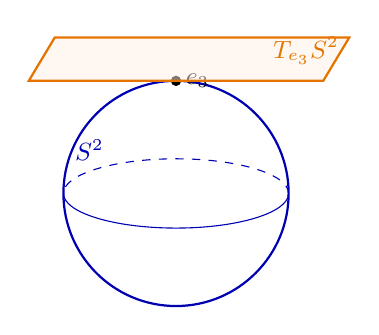
\begin{tikzpicture}[scale=1.1]
  \draw[blue!70!black, thick] (0,0) circle (1.3);
  \draw[blue!70!black, dashed] (1.3,0) arc (0:180:1.3 and 0.4);
  \draw[blue!70!black] (-1.3,0) arc (180:360:1.3 and 0.4);
  \node[blue!70!black, font=\small] at (-1.0,0.5) {$S^2$};

  \fill (0,1.3) circle (1.7pt) node[right, font=\small] {$e_3$};
  \draw[orange!90!black, thick, fill=orange!10, fill opacity=0.5]
    (-1.7,1.3) -- (1.7,1.3) -- (2.0,1.8) -- (-1.4,1.8) -- cycle;
  \node[orange!90!black, font=\small] at (1.5,1.65) {$T_{e_3}S^2$};
\end{tikzpicture}
\end{center}

% Quelle: Diego Torres Tejeda/Notes - 30.03 - Diego Torres Tejeda.pdf, p. 2 -- Sonnet 5 (Medium)
% Corsin defines T_pM only via a parametrization; the curve description below is Diego's. (Was
% an ainote until 2026-08-09. The mathematics is the proposition, and who-wrote-which-definition
% is editor-facing by Test 2 in style.md.)
\Cref{def:tangent_space} builds $T_pM$ out of a parametrization, so the space is pinned down by a
formula rather than by what its elements are. There is an equivalent description that says what
they are. A vector is tangent to $M$ at $p$ exactly when some curve running inside $M$ passes
through $p$ with that velocity, which is both how tangent vectors are usually pictured and the
quicker test in practice, since no parametrization need be written down.

\begin{proposition}[Tangent space via curves]
\label{prop:tangent_space_via_curves}
Let $M^m \subseteq \mathbb{R}^n$ be a $C^k$ submanifold ($k\geq1$) and $p \in M$. Then
\[T_pM = \big\{\gamma'(0) : \gamma \in C^1\big((-\varepsilon,\varepsilon), \mathbb{R}^n\big),\ \varepsilon>0,\ \gamma(t) \in M \text{ for all } t,\ \gamma(0)=p\big\}.\]
\end{proposition}

\begin{proof}
Let $\Phi : U \to V$ be a submanifold chart at $p$ (\cref{def:submanifold}), so
$\Phi(U\cap M) = (\mathbb{R}^m\times\{0\})\cap V$ and $\Phi(p)=0$; equivalently, let
$f := \Phi^{-1}|_{(\mathbb{R}^m\times\{0\})\cap V}$ be the corresponding local parametrization
(\cref{thm:local_parametrization}), $f(q)=p$.

\textbf{($\subseteq$)} Let $v \in T_pM = Df_q(\mathbb{R}^m)$, say $v = Df_q(w)$. The curve
$\gamma(t) := f(q+tw)$, defined for $t$ small enough that $q+tw$ stays in $f$'s domain, satisfies
$\gamma(t) \in M$ for all such $t$, $\gamma(0) = p$, and by the chain rule
$\gamma'(0) = Df_q(w) = v$.

\textbf{($\supseteq$)} Let $\gamma$ be a curve as in the statement. Since $\Phi$ is a
diffeomorphism with $\Phi(\gamma(t)) \in \mathbb{R}^m\times\{0\}$ for all $t$ near $0$, write
$\Phi\circ\gamma =: (\eta,0)$ with $\eta \in C^1\big((-\varepsilon,\varepsilon),\mathbb{R}^m\big)$.
Then $\gamma = \Phi^{-1}(\eta,0) = f(\eta(\cdot))$ near $0$ (shrinking $U$ if necessary so that
$f$ is defined on all of $\eta$'s image), so by the chain rule,
\[\gamma'(0) = Df_{\eta(0)}\big(\eta'(0)\big) \in Df_q(\mathbb{R}^m) = T_pM\]
(using $\eta(0)=q$, since $\Phi(p)=0=\Phi(f(q))$ and $\Phi$ is injective).
\end{proof}

% Sonnet 5 (Medium)
\begin{center}
\begin{tikzpicture}[>=Latex, scale=1.1]
  \draw[blue!70!black, thick] plot[smooth] coordinates
    {(-1.8,-0.8) (-0.8,0.6) (0.4,-0.2) (1.4,0.9) (2.2,0.1)};
  \coordinate (P) at (0.4,-0.2);
  \fill (P) circle (1.7pt) node[below, font=\small] {$p=\gamma(0)$};
  \draw[orange!90!black, thick, ->] (P) -- ++(0.9,0.75) node[right, font=\small] {$\gamma'(0)$};
\end{tikzpicture}
\end{center}

% Source: Jérôme Paschoud/Notizen/Woche 8.1 Tangentialräume und Jordan Mass.pdf, p. 1
% Generator: Gemini 3.1 Pro (High)
\begin{remark}[Four representations of the tangent space]
\label{rem:four_representations_tangent_space}
Depending on how a $m$-dimensional submanifold $M \subseteq \mathbb{R}^n$ is locally described near $p$, its tangent space $T_pM$ can be computed algebraically in four equivalent ways:
\begin{itemize}
  \item \textbf{Diffeomorphism} (from the definition, $\Psi(p)=0$): $T_pM = (D\Psi_p)^{-1}(\mathbb{R}^m \times \{0\})$.
  \item \textbf{Implicit representation} ($M = F^{-1}\{0\}$): $T_pM = \ker(DF_p)$.
  \item \textbf{Parametric representation} (local parametrization $g$ with $g(q)=p$): $T_pM = Dg_q(\mathbb{R}^m)$.
  \item \textbf{Graph representation} (graph of $h$, $p=(z, h(z))$): $T_pM = \{(w, Dh_z(w)) \mid w \in \mathbb{R}^m\}$.
\end{itemize}
These algebraic descriptions are all equivalent to the geometric description via velocities of curves (\cref{prop:tangent_space_via_curves}).
\end{remark}

\subsection{Normal space}

% Source: Corsin Nick/Class Notes/Week 7.pdf, pp. 9--10
Suppose $F : U \to \mathbb{R}^{n-m}$ is an implicit representation of $M^m = F^{-1}\{0\}$ (via the
regular value theorem) and $f : V^m \to M$ is a local parametrization, $M$ a submanifold. Then, by
definition,
\begin{enumerate}[label=\textbf{\arabic*.}]
  \item The Jacobian matrix:
\[ \Jac F(x) = \begin{pmatrix} \nabla F_1(x) \longrightarrow \\ \vdots \\ \nabla F_{n-m}(x) \longrightarrow \end{pmatrix} \]
    has full rank, i.e., $\{\nabla F_i(x)\}_{i=1,\dots,n-m}$ are linearly independent;
  \item $T_{f(q)}M = \operatorname{span}\{\partial_if(q)\}$, as above;
  \item $F(f(x)) = 0$ for all $x \in V$, since $f(x) \in M = F^{-1}\{0\}$.
\end{enumerate}
From \textbf{3}, it follows that
\begin{align*}
\Jac(F\circ f)(q)
  &= \Jac F(f(q))\cdot\Jac f(q) \\
  &= \begin{pmatrix} \nabla F_1(f(q)) \longrightarrow \\ \vdots \\ \nabla F_{n-m}(f(q)) \longrightarrow \end{pmatrix}
     \begin{pmatrix} \dfrac{\partial f}{\partial q_1} & \cdots & \dfrac{\partial f}{\partial q_m}\end{pmatrix}
   \;=\; 0.
\end{align*}
Now, since $\big(\Jac F(f(q))\cdot\Jac f(q)\big)_{ij} = \langle \nabla F_i(f(q)), \partial_jf(q)\rangle = 0$
for all $i=1,\dots,n-m$, $j=1,\dots,m$, the vectors $\nabla F_i(f(q))$ are perpendicular, that is,
\newterm{normal}, to $T_{f(q)}M$. Since by \textbf{1} we have $n-m$ linearly independent vectors
normal to the $m$-dimensional plane $T_{f(q)}M$, we can define:

\begin{definition}[Normal space]
\label{def:normal_space}
Let $M^m \subseteq \mathbb{R}^n$ be a submanifold and $F : U^n \to \mathbb{R}^{n-m}$ an implicit
representation, $M = F^{-1}\{0\}$. Then the \newterm{normal space} \germanfor{Normalraum} of
$M$ at $p \in M$ is
\[N_pM := \operatorname{span}\{\nabla F_1(p),\dots,\nabla F_{n-m}(p)\}.\]
\end{definition}

\begin{example}[Normal space to the sphere]
Represent $S^2$ implicitly: $S^2 = F^{-1}\{1\} = \{(x,y,z)\in\mathbb{R}^3 : F(x,y,z)=1\}$ where
$F(x,y,z) = x^2+y^2+z^2$. We determine $N_{e_3}S^2$:
\[\nabla F(0,0,1) = (2x,2y,2z)\big|_{(x,y,z)=(0,0,1)} = 2e_3.\]
So, $N_{e_3}S^2 = \operatorname{span}\{e_3\} = \{0\}\times\mathbb{R}$.
\end{example}

% Generator: Claude Opus 5 (High) --- the example above is the $n=3$, $F = \lvert x\rvert^2$
% instance of a general fact worth stating once, since it is what makes the Lagrange condition
% of \cref{prop:constrained_optimization} geometric rather than algebraic.
\begin{proposition}[The gradient is normal to the level set]
\label{prop:gradient_orthogonality_level_sets}
Let $U \subseteq \mathbb{R}^n$ be open, $g \in C^1(U,\mathbb{R})$, and let
$S := \{x \in U : g(x) = c\}$ for some $c \in \mathbb{R}$. If $\nabla g(x_0) \neq 0$ at a point
$x_0 \in S$, then near $x_0$ the set $S$ is an $(n-1)$-dimensional submanifold and
\[N_{x_0}S = \operatorname{span}\{\nabla g(x_0)\}.\]
In particular the normal space is a \emph{line}, and the affine \emph{tangent} hyperplane to $S$
at $x_0$ is $\{x \in \mathbb{R}^n : \langle x - x_0,\ \nabla g(x_0)\rangle = 0\}$.
\end{proposition}

\begin{proof}
That $S$ is a submanifold of dimension $n-1$ near $x_0$ is \cref{thm:regular_value_theorem},
since $\nabla g(x_0) \neq 0$ says exactly that $Dg_{x_0} : \mathbb{R}^n \to \mathbb{R}$ is
surjective. For the normal space, let $v \in T_{x_0}S$ and pick a $C^1$ curve
$\gamma : (-\varepsilon,\varepsilon) \to S$ with $\gamma(0) = x_0$ and $\gamma'(0) = v$. Then
$g \circ \gamma \equiv c$, so differentiating at $t=0$ with the chain rule along a path
(\cref{sec:chain_rule_along_path}) gives
\[0 = \frac{d}{dt}\Big|_{t=0}g(\gamma(t)) = \big\langle \nabla g(x_0),\ v\big\rangle.\]
Hence $\nabla g(x_0) \perp T_{x_0}S$, that is,
$\operatorname{span}\{\nabla g(x_0)\} \subseteq N_{x_0}S$. Both are subspaces of dimension
$n - \dim T_{x_0}S = n-(n-1) = 1$, so they are equal.
\end{proof}

% Supplement: Sascha Brack/Class Notes/Week_08_Notes_Monday.pdf, pp. 3--4
\begin{example}[Tangent and normal vectors via parametrization]
\label{ex:tangent_normal_parametrized_sphere}
For a parametrized surface $f : V \to \mathbb{R}^3$, the tangent space at $p = f(x)$ is $T_pM = \operatorname{span}\{\partial_1 f(x), \partial_2 f(x)\}$. A normal vector can be found via the cross product: $\vec{n} = \partial_1 f(x) \times \partial_2 f(x)$.

Let us apply this to the sphere $S^2$ using spherical coordinates:
\[\Phi(\theta,\varphi) = \begin{pmatrix} \sin\theta\cos\varphi \\ \sin\theta\sin\varphi \\ \cos\theta \end{pmatrix}, \qquad (\theta,\varphi) \in (0,\pi) \times (-\pi,\pi).\]
(Note that the image of $\Phi$ is the unit sphere minus a \qt{thin slice}, namely the meridian where $\varphi = \pm\pi$ together with the two poles where $\theta \in \{0,\pi\}$.)
The tangent space $T_{\Phi(\theta,\varphi)} S^2$ is spanned by the partial derivatives:
\[
\partial_\theta \Phi(\theta,\varphi) = \begin{pmatrix} \cos\theta\cos\varphi \\ \cos\theta\sin\varphi \\ -\sin\theta \end{pmatrix}, \qquad
\partial_\varphi \Phi(\theta,\varphi) = \begin{pmatrix} -\sin\theta\sin\varphi \\ \sin\theta\cos\varphi \\ 0 \end{pmatrix}.
\]
A normal vector is given by their cross product:
% Split across three lines: as one display this overflowed the text block by 70pt, which the
% house style forbids for chains of matrix blocks.
\begin{align*}
\vec{n} = \partial_\theta \Phi \times \partial_\varphi \Phi
  &= \begin{pmatrix} \cos\theta\cos\varphi \\ \cos\theta\sin\varphi \\ -\sin\theta \end{pmatrix}
     \times
     \begin{pmatrix} -\sin\theta\sin\varphi \\ \sin\theta\cos\varphi \\ 0 \end{pmatrix} \\
  &= \begin{pmatrix} \sin^2\theta\cos\varphi \\ \sin^2\theta\sin\varphi \\
       \sin\theta\cos\theta\cos^2\varphi + \sin\theta\cos\theta\sin^2\varphi \end{pmatrix} \\
  &= \sin\theta \begin{pmatrix} \sin\theta\cos\varphi \\ \sin\theta\sin\varphi \\ \cos\theta \end{pmatrix}.
\end{align*}
Its length is $|\vec{n}| = \sin\theta$ (since $\sin\theta > 0$ for $\theta \in (0,\pi)$).
The unit normal vector is therefore
\[
\nu(\theta,\varphi) := \frac{\vec{n}}{|\vec{n}|} = \begin{pmatrix} \sin\theta\cos\varphi \\ \sin\theta\sin\varphi \\ \cos\theta \end{pmatrix} = \Phi(\theta,\varphi).
\]
This confirms that the outward normal vector at a point on the unit sphere is precisely the position vector of that point.
\end{example}

% Sonnet 5 (Medium) --- FIG-W07-06
\begin{center}
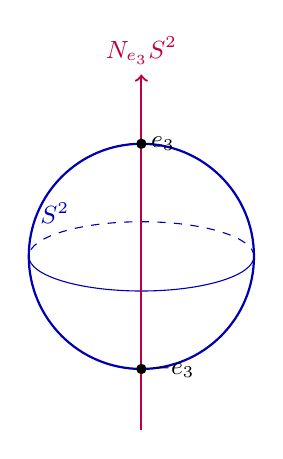
\begin{tikzpicture}[scale=1.1]
  \draw[blue!70!black, thick] (0,0) circle (1.3);
  \draw[blue!70!black, dashed] (1.3,0) arc (0:180:1.3 and 0.4);
  \draw[blue!70!black] (-1.3,0) arc (180:360:1.3 and 0.4);
  \node[blue!70!black, font=\small] at (-1.0,0.5) {$S^2$};

  \draw[purple, thick, ->] (0,-2.0) -- (0,2.1) node[above, font=\small] {$N_{e_3}S^2$};
  \fill (0,1.3) circle (1.7pt) node[right, font=\small] {$e_3$};
  \fill (0,-1.3) circle (1.7pt) node[right, font=\small] {$-e_3$};
\end{tikzpicture}
\end{center}


% --- exercise relocated here from the dissolved sheet 7 ---

% Originally: content/week-07.tex, \exercisesheet{7}, problem 7.6
% Source: exercises/Ex7_Analysis2_eng.pdf

\begin{exercise}[7.6 --- Spherical coordinates \textnormal{(important)}]
\label{ex:7.6}
The mapping $\Phi : (0,\infty)\times(0,\pi)\times(-\pi,\pi) \to \mathbb{R}^3$ defined by
\[\Phi(r,\theta,\varphi) = \begin{pmatrix} r\sin\theta\cos\varphi \\ r\sin\theta\sin\varphi \\ r\cos\theta \end{pmatrix}\]
is called \textit{spherical coordinates}.
\begin{enumerate}[label=\textbf{\arabic*.}]
  \item Sketch the images of $r \mapsto \Phi(r,\theta_0,\varphi_0)$, $\theta \mapsto
    \Phi(r_0,\theta,\varphi_0)$ and $\varphi \mapsto \Phi(r_0,\theta_0,\varphi)$ for some fixed
    $r_0 \in (0,\infty)$, $\theta_0 \in (0,\pi)$, $\varphi_0 \in (-\pi,\pi)$.
  \item What is the image of $\Phi$?
  \item Show that $\det(D_{(r,\theta,\varphi)}\Phi) = r^2\sin\theta$ holds.
  \item Conclude that the mapping $\Phi$ is a diffeomorphism onto its image.
\end{enumerate}
\end{exercise}

% Originally: content/week-07.tex, \section{Solutions}

\section{Solutions}
\label{sec:submanifolds_solutions}

% Transition: Claude Opus 5 (High)
Not every solution in this chapter is collected here. \Cref{ex:dimension_submanifold_system}
(\cpageref{ex:dimension_submanifold_system}) and \cref{ex:submanifold_matrices_rank1}
(\cpageref{ex:submanifold_matrices_rank1}) are solved where they appear.

\begin{ainote}
Corsin's notes for this material cover only the theory (submanifolds, the regular value and local
parametrization theorems, tangent and normal spaces), with no page working out any of the
official-sheet exercises, so all solutions below are original. Those answering a problem from
Sheet 7 have been checked against \texttt{exercises/Sol7\_Analysis2\_eng.pdf}, and no divergence
from the official solutions was found. The exam problems mined into this chapter come from papers
that ship no key at all, so those solutions rest on independent derivation alone.
\end{ainote}

\begin{exercisesolution}[Solution to \cref{ex:7.6}]
% Generator: Claude Sonnet 5 (Medium)
\begin{enumerate}[label=\textbf{(\alph*)}]
  \item Fixing $\theta_0,\varphi_0$, the image of $r \mapsto \Phi(r,\theta_0,\varphi_0)$ is the
    radial half-line through the point $p_0 := (\sin\theta_0\cos\varphi_0,
    \sin\theta_0\sin\varphi_0, \cos\theta_0)$ on the unit sphere, i.e., $\{rp_0 : r \in
    (0,\infty)\}$. Fixing $r_0,\varphi_0$, the image of $\theta \mapsto \Phi(r_0,\theta,\varphi_0)$
    is a semicircle of radius $r_0$ from the north pole to the south pole (excluding the poles),
    at longitude $\varphi_0$. Fixing $r_0,\theta_0$, the image of $\varphi \mapsto
    \Phi(r_0,\theta_0,\varphi)$ is a circle of latitude of radius $r_0\sin\theta_0$ at height
    $r_0\cos\theta_0$ (excluding the point at $\varphi = \pm\pi$).
  \item For each fixed $r$, the image sweeps out the sphere of radius $r$ minus the half-plane
    at $\varphi = \pm\pi$ (the \emph{anti}-meridian, since the prime meridian is $\varphi = 0$).
    Overall,
    \[\operatorname{im}(\Phi) = \mathbb{R}^3\setminus\big((-\infty,0]\times\{0\}\times\mathbb{R}\big).\]
  \item Computing,
    \[D_{(r,\theta,\varphi)}\Phi = \begin{pmatrix} \sin\theta\cos\varphi & r\cos\theta\cos\varphi & -r\sin\theta\sin\varphi \\ \sin\theta\sin\varphi & r\cos\theta\sin\varphi & r\sin\theta\cos\varphi \\ \cos\theta & -r\sin\theta & 0 \end{pmatrix},\]
    hence, expanding along the last row,
    \[\begin{aligned}
    \det(D_{(r,\theta,\varphi)}\Phi) &= r^2\sin\theta\cos^2\theta\cos^2\varphi+r^2\sin^3\theta\sin^2\varphi+r^2\sin\theta\cos^2\theta\sin^2\varphi+r^2\sin^3\theta\cos^2\varphi \\
    &= r^2\big(\sin\theta\cos^2\theta+\sin^3\theta\big) = r^2\sin\theta.
    \end{aligned}\]
  \item Since $r \in (0,\infty)$ and $\theta \in (0,\pi)$, $r^2\sin\theta$ is never $0$, so
    $\Jac\Phi(r,\theta,\varphi)$ is everywhere invertible and $\Phi$ is a local diffeomorphism by
    \Cref{thm:inverse_function_theorem}. To see it is a \textbf{global} diffeomorphism onto its
    image, it remains to check $\Phi$ is injective: if $\Phi(r_1,\theta_1,\varphi_1) =
    \Phi(r_2,\theta_2,\varphi_2)$, then $r_1=r_2$ follows by taking the norm of both sides; since
    $\cos : (0,\pi) \to (-1,1)$ is injective, the third coordinate gives $\theta_1=\theta_2$;
    finally $(\cos\varphi,\sin\varphi)$ with $\varphi \in (-\pi,\pi)$ determines a unique point on
    the unit circle, so $\varphi_1=\varphi_2$. Hence $\Phi$ is injective, and (being a local
    diffeomorphism everywhere on its domain) a diffeomorphism onto its image.
\end{enumerate}
\end{exercisesolution}

\begin{exercisesolution}[Proof of \cref{ex:submanifold_quadric_tangent_space}]
% Generator: Gemini 3.6 Flash (High)
% Correction: Claude Opus 5 (High) --- ^T -> \transp throughout, \implies replaced by prose, and the
% check that p lies on M added: the tangent space computation presupposes it.
\begin{enumerate}[label=\textbf{(\alph*)}]
  \item Define the smooth function $F : \mathbb{R}^3 \to \mathbb{R}$,
    $F(x_1,x_2,x_3) := x_1 x_2 + x_2 x_3 + x_1 x_3 - 1$, so that $M = F^{-1}(0)$. Its gradient is
\[\nabla F(x) = (x_2+x_3,\; x_1+x_3,\; x_1+x_2)\transp .\]
    Suppose $\nabla F(x) = 0$. Adding the three equations $x_2+x_3 = x_1+x_3 = x_1+x_2 = 0$ gives
    $2(x_1+x_2+x_3) = 0$, and subtracting each equation in turn then forces $x_1 = x_2 = x_3 = 0$.
    But $F(0,0,0) = -1 \neq 0$, so the origin is not in $M$. Hence $\nabla F$ is non-zero at every
    point of $M$, which is to say $0$ is a regular value of $F$. By the regular value theorem
    (\cref{thm:regular_value_theorem}), $M$ is a smooth submanifold of $\mathbb{R}^3$ of dimension
    $3 - 1 = 2$.

  \item First, $p = (-1,2,3)$ does lie on $M$: indeed $(-1)(2) + (2)(3) + (-1)(3) = -2 + 6 - 3 = 1$.
    At this point,
\[\nabla F(-1,2,3) = (2+3,\; -1+3,\; -1+2)\transp = (5, 2, 1)\transp .\]
    The tangent space is the kernel of $DF(p)$, equivalently the orthogonal complement of
    $\nabla F(p)$:
\[T_p M = \left\{(v_1, v_2, v_3)\transp \in \mathbb{R}^3 \;\middle|\; 5v_1 + 2v_2 + v_3 = 0\right\}.\]
    Reading $v_3$ off from $v_1$ and $v_2$ gives two independent solutions: taking $(v_1,v_2) =
    (1,0)$ yields $v_3 = -5$, and taking $(v_1,v_2) = (0,1)$ yields $v_3 = -2$. Hence
\[\left\{\begin{pmatrix} 1 \\ 0 \\ -5 \end{pmatrix}, \begin{pmatrix} 0 \\ 1 \\ -2 \end{pmatrix}\right\}\]
    is a basis of $T_p M$; the two vectors are independent because their first two components
    already are, and there are two of them, matching $\dim T_p M = 2$.
\end{enumerate}
\begin{ainote}
The official solution gives the basis $\left\{(2,-5,0)\transp,\ (1,0,-5)\transp\right\}$, which
looks different from the one above but is not a disagreement: both are bases of the same plane
$\ker(5,2,1)$, and each vector of either list satisfies $5v_1+2v_2+v_3 = 0$. \qt{Give a basis} has
infinitely many correct answers, and no canonical one --- so when checking work against a master
solution here, verify that each vector is annihilated by $\nabla F(p)$ and that the two are
independent, rather than comparing entries. The two lists even share the vector $(1,0,-5)\transp$.
The official solution also invokes the constant rank theorem via surjectivity of $D_xF$ where we
cite the regular value theorem (\cref{thm:regular_value_theorem}); for a real-valued $F$ these say
the same thing, since a linear map $\mathbb{R}^3 \to \mathbb{R}$ is surjective precisely when its
gradient is non-zero.
\end{ainote}
\end{exercisesolution}

\begin{exercisesolution}[Solution of \cref{ex:image_of_segment_submanifold}]
% Generator: Claude Opus 5 (High)
For $\alpha = 0$ the determinant computed in \cref{ex:local_diffeo_parameter_alpha} is
$-16 \neq 0$, so fix $r > 0$ small enough that $\Phi$ restricted to $B_r(0,0)$ is a
$C^1$-diffeomorphism onto the open set $\Phi(B_r(0,0))$. Write
\[S := \{(x,y) \in B_r(0,0) \mid y = 0\} = (-r,r) \times \{0\}\]
for the segment in question. It is itself a $1$-dimensional $C^1$ submanifold of $\mathbb{R}^2$:
given $p = (a,0) \in S$, the translation $\Psi(x,y) := (x-a,\, y)$ is a diffeomorphism from
$U_p := B_r(0,0)$ onto the open set $V := \Psi(U_p)$, it sends $p$ to $0$, and
$\Psi(U_p \cap S) = (\mathbb{R}\times\{0\}) \cap V$.
\begin{enumerate}[label=\textbf{(\alph*)}]
  \setcounter{enumi}{3}
  \item \textbf{True.} Apply \cref{prop:diffeomorphism_preserves_submanifold} to the
    $C^1$-diffeomorphism $\Phi|_{B_r(0,0)} : B_r(0,0) \to \Phi(B_r(0,0))$ and to $S$. The image
    $\Phi(S)$ is a $C^1$ submanifold of $\mathbb{R}^2$ of dimension $1$.
  \item \textbf{False.} By \textbf{(d)} the set is $1$-dimensional, and no non-empty set is a
    submanifold of two different dimensions at once. Independently of that: a $2$-dimensional
    submanifold of $\mathbb{R}^2$ is an \emph{open} subset of $\mathbb{R}^2$, because a chart with
    $m = n = 2$ reads $\Psi(U \cap M) = V = \Psi(U)$, so $U \cap M = U$ and $M$ contains the open
    neighbourhood $U$ of each of its points. But $\Phi(S)$ is not open. Its complement in
    $\Phi(B_r(0,0))$ is the image of $B_r(0,0) \setminus S$, which is dense in $B_r(0,0)$, and a
    homeomorphism carries dense sets to dense sets, so every point of $\Phi(S)$ is a limit of
    points outside it.
\end{enumerate}
\begin{remark}[The pair is a dimension check, not a submanifold check]
The two items ask about the same set, so at most one can be true, and the real question is which
number a diffeomorphism is allowed to change. It changes none:
\cref{rem:dimension_is_a_diffeomorphism_invariant} is the whole content of the block. The picture
that makes \textbf{(e)} tempting is that $\Phi$ maps a two-dimensional ball onto a two-dimensional
region, so its image \qt{fills out} the plane. It does, but the segment does not, and it is the
segment being transported.
\end{remark}
\end{exercisesolution}

% Generator: Claude Opus 5 (High)
% No solution key ships with the Jossen papers, so this is an independent derivation.
\begin{exercisesolution}[\cref{ex:orthogonal_group_submanifold}]
\begin{enumerate}[label=\textbf{(\alph*)}]
  \item With $A = \left(\begin{smallmatrix} a & b \\ c & d\end{smallmatrix}\right)$,
\[AA\transp = \begin{pmatrix} a & b \\ c & d \end{pmatrix}
              \begin{pmatrix} a & c \\ b & d \end{pmatrix}
            = \begin{pmatrix} a^2+b^2 & ac+bd \\ ac+bd & c^2+d^2 \end{pmatrix},\]
    so in the coordinates of the statement
\[F(a,b,c,d) = \big(a^2+b^2,\ ac+bd,\ ac+bd,\ c^2+d^2\big).\]
    Every component is a polynomial, hence $F$ is smooth.

  \item $(AA\transp)\transp = (A\transp)\transp A\transp = AA\transp$, so $F(A)$ is symmetric for
    every $A$. This is already visible in the coordinate formula: the second and third components
    of $F$ are the same function.

  \item Differentiating the four components with respect to $a,b,c,d$ in turn,
\[\Jac F(a,b,c,d) = \begin{pmatrix}
  2a & 2b & 0 & 0 \\
  c & d & a & b \\
  c & d & a & b \\
  0 & 0 & 2c & 2d
\end{pmatrix}.\]

  \item The second and third rows coincide for every $A$, so $\rank \Jac F(A) \le 3$ always. To see
    that equality holds on $\Orth_2(\mathbb{R})$, note that $AA\transp = \id$ says exactly that the
    two rows $u := (a,b)$ and $v := (c,d)$ of $A$ are orthonormal. Suppose
\[\alpha(2a,2b,0,0) + \beta(c,d,a,b) + \gamma(0,0,2c,2d) = 0.\]
    Its first two coordinates read $2\alpha u + \beta v = 0$, and $u,v$ are linearly independent,
    so $\alpha = \beta = 0$. The last two then read $2\gamma v = 0$, so $\gamma = 0$ as well. The
    three distinct rows are therefore independent and the rank is exactly $3$.

    This is why \cref{thm:regular_value_theorem} cannot be applied to $F$ as a map
    $\mathbb{R}^4 \to \mathbb{R}^4$: the theorem needs $D_AF$ to be \emph{surjective}, that is of
    rank $4$, and the rank is $3$ at every point of $\Orth_2(\mathbb{R})$. Nor is this a defect of
    the particular level: by \textbf{(b)} the image of $F$ lies in a three-dimensional subspace, so
    $D_AF$ is nowhere surjective, for any $A$ whatsoever.

  \item Identify $\operatorname{Sym}_2(\mathbb{R}) \cong \mathbb{R}^3$ by
    $\left(\begin{smallmatrix} p & q \\ q & s\end{smallmatrix}\right) \mapsto (p,q,s)$ and let
\[\widetilde F : \mathbb{R}^4 \to \mathbb{R}^3, \qquad
  \widetilde F(a,b,c,d) := \big(a^2+b^2,\ ac+bd,\ c^2+d^2\big),\]
    which is $F$ with the duplicated component dropped. Then
    $\Orth_2(\mathbb{R}) = \widetilde F^{-1}\{(1,0,1)\}$, and
\[\Jac \widetilde F(a,b,c,d) = \begin{pmatrix}
  2a & 2b & 0 & 0 \\
  c & d & a & b \\
  0 & 0 & 2c & 2d
\end{pmatrix}\]
    has rank $3$ at every point of $\Orth_2(\mathbb{R})$, by the computation in \textbf{(d)}. So
    $(1,0,1)$ is a regular value of $\widetilde F$, and the regular value theorem makes
    $\Orth_2(\mathbb{R})$ a smooth submanifold of $\mathbb{R}^4 = \operatorname{Mat}_2(\mathbb{R})$
    of dimension $4 - 3 = 1$.

  \item By \cref{prop:gradient_orthogonality_level_sets} applied to each of the three defining
    equations, or directly from the description of the tangent space to a regular level set,
    $T_{\id}\Orth_2(\mathbb{R}) = \ker \Jac \widetilde F(\id)$. At
    $(a,b,c,d) = (1,0,0,1)$,
\[\Jac \widetilde F(1,0,0,1) = \begin{pmatrix}
  2 & 0 & 0 & 0 \\
  0 & 1 & 1 & 0 \\
  0 & 0 & 0 & 2
\end{pmatrix},\]
    so a vector $(v_1,v_2,v_3,v_4)$ lies in the kernel precisely when $v_1 = 0$, $v_4 = 0$ and
    $v_2 + v_3 = 0$. Hence
\[T_{\id}\Orth_2(\mathbb{R}) = \operatorname{span}\left\{
  \begin{pmatrix} 0 \\ 1 \\ -1 \\ 0\end{pmatrix}\right\}
  = \operatorname{span}\left\{\begin{pmatrix} 0 & 1 \\ -1 & 0\end{pmatrix}\right\},\]
    a line, in agreement with $\dim \Orth_2(\mathbb{R}) = 1$ from \textbf{(e)}. Using the full
    $4\times4$ Jacobian of \textbf{(c)} gives the same kernel, since the repeated row imposes no
    new condition.
\end{enumerate}
\begin{remark}[The tangent space names the answer]
The line found in \textbf{(f)} consists of the \emph{antisymmetric} $2\times2$ matrices, and that
is not a coincidence: differentiating $A(t)A(t)\transp = \id$ along any curve in
$\Orth_2(\mathbb{R})$ through $\id$ gives $\dot A(0) + \dot A(0)\transp = 0$. The same computation
in $n$ dimensions gives $\dim\Orth_n(\mathbb{R}) = \binom{n}{2}$, the dimension of the
antisymmetric matrices, which for $n=2$ is $1$.

That $\Orth_2(\mathbb{R})$ is one-dimensional is worth pausing on, because it is easy to expect
more. Writing $u = (\cos\theta,\sin\theta)$ for the first row, orthonormality leaves exactly two
choices of second row, so $\Orth_2(\mathbb{R})$ is a disjoint union of two circles: the rotations
$\det A = 1$ and the reflections $\det A = -1$. A submanifold need not be connected, and the
regular value theorem never claims it is.

Set against \cref{ex:submanifold_matrices_rank1}, which lives in the same $\mathbb{R}^4$, the
contrast is instructive. There a single scalar equation cut out a three-dimensional submanifold and
the regular value theorem applied as it stands. Here the naive count would suggest
$4 - 4 = 0$ dimensions, and it is wrong precisely because the four equations $AA\transp = \id$ are
not independent: one of them is a duplicate. Counting equations is only a shortcut for computing a
rank, and when the shortcut and the rank disagree it is the rank that is right.
\end{remark}
\end{exercisesolution}

\begin{exercisesolution}[Solution to \cref{ex:operations_preserving_submanifolds}]
% Generator: Claude Opus 5 (High) --- the four statements are the examiner's; the working, the
% counterexample in (b) and the remark are written for these notes. Probeprfg1 ships no key.
Throughout, \qt{submanifold} is used in the sense of \cref{def:submanifold}: locally
straightenable by a diffeomorphism of the ambient space.
\begin{enumerate}[label=\textbf{(\alph*)}]
  \item \textbf{True}, and there is nothing to prove beyond intersecting with one more open set.
    Being open in $M$ means $N = M \cap W$ for some open $W \subseteq \mathbb{R}^n$. Fix $p \in
    N$ and take a submanifold chart $\Psi : U_p \to V$ for $M$ at $p$. Replacing $U_p$ by
    $U_p \cap W$, which is still an open neighbourhood of $p$, turns it into a submanifold chart
    for $N$ at $p$ of the same dimension. The definition is local, so shrinking the neighbourhood
    costs nothing.
  \item \textbf{False}, and this is the one that has to be met rather than reasoned about.
    In $\mathbb{R}^2$ take
    \[M := \{(x,0) \mid x > 0\}, \qquad N := \{(0,y) \mid y \in \mathbb{R}\}.\]
    They are disjoint, since every point of $M$ has $x > 0$ and every point of $N$ has $x = 0$,
    and each is a $1$-dimensional submanifold: $M$ is an open subset of the $x$-axis, so
    part \textbf{(a)} applies, and $N$ is a line.

    But $M \cup N$ is not a submanifold at the origin. Every ball $B_\varepsilon(0,0)$ meets it
    in a segment of the $y$-axis together with a half-open segment running right, and deleting
    the origin from that set leaves \emph{three} connected pieces, whereas deleting a point from
    a straightened $(\mathbb{R}\times\{0\})\cap V$ leaves two. No diffeomorphism can change the
    number of pieces, so no submanifold chart exists at $(0,0)$.

    What goes wrong is that disjointness is not enough: the two pieces are disjoint but one of
    them accumulates on the other. Requiring instead that $M$ and $N$ have disjoint
    \emph{closures} makes the statement true, and then each point of the union has a
    neighbourhood meeting only one of the two.
  \item \textbf{True}, and it is the chart definition again. Fix $(p,q) \in M \times N$ and take
    submanifold charts $\Psi : U_p \to V$ for $M$ and $\Xi : U_q \to W$ for $N$, with
    $\Psi(U_p \cap M) = (\mathbb{R}^k\times\{0\})\cap V$ and
    $\Xi(U_q \cap N) = (\mathbb{R}^l\times\{0\})\cap W$. Then $\Psi\times\Xi$ is a
    diffeomorphism of the open set $U_p\times U_q \subseteq \mathbb{R}^{m+n}$ onto $V\times W$,
    and it carries $(U_p\times U_q) \cap (M\times N)$ onto
    \[\big((\mathbb{R}^k\times\{0\})\cap V\big) \times \big((\mathbb{R}^l\times\{0\})\cap W\big).\]
    Composing with the permutation of coordinates that gathers the $k$ and the $l$ live
    directions together, which is linear and invertible and hence a diffeomorphism, turns this
    into $(\mathbb{R}^{k+l}\times\{0\}) \cap (V\times W)$. That is a submanifold chart of
    dimension $k+l$.
  \item \textbf{True}, and the hypothesis on the tangent spaces is exactly what is needed. Fix
    $p \in M \cap N$. Each of $M$ and $N$ is locally a level set, and \cref{def:submanifold}
    supplies this directly: a submanifold chart $\Psi : U \to V$ for $M$ at $p$ satisfies
    $\Psi(U \cap M) = (\mathbb{R}^{n-1}\times\{0\}) \cap V$, so its last component
    $F := \Psi_n$ is $C^1$ with $M \cap U = F^{-1}\{0\}$, and $\nabla F(p) \neq 0$ because it is
    a row of the invertible matrix $\Jac\Psi(p)$. Do the same for $N$, shrink to a common
    neighbourhood, and write $G$ for its function. So
    \[M \cap U = F^{-1}\{0\}, \quad \nabla F(p) \neq 0, \qquad
      N \cap U = G^{-1}\{0\}, \quad \nabla G(p) \neq 0 .\]
    By \cref{prop:gradient_orthogonality_level_sets}, $T_pM$ has $\nabla F(p)$ as its
    normal line, and likewise for $N$. Two hyperplanes in $\mathbb{R}^n$ coincide precisely when
    their normal lines do, so $T_pM \neq T_pN$ says exactly that $\nabla F(p)$ and $\nabla G(p)$
    are linearly independent.

    That makes $H := (F,G) : U \to \mathbb{R}^2$ a map whose Jacobian at $p$ has the two
    independent rows $\nabla F(p)\transp$ and $\nabla G(p)\transp$, hence rank $2$, so $DH_p$ is
    surjective. Full rank is an open condition, so after shrinking $U$ it holds throughout, and
    \cref{thm:regular_value_theorem} makes
    \[H^{-1}\{0\} = (M\cap U) \cap (N \cap U) = (M\cap N)\cap U\]
    a submanifold of dimension $n-2$. As $p$ was arbitrary, $M \cap N$ is one.
\end{enumerate}

\begin{remark}[Transversality is the name of the hypothesis in \textbf{(d)}]
Two submanifolds are said to meet \newterm{transversally} at $p$ if their tangent spaces together
span the ambient space, $T_pM + T_pN = \mathbb{R}^n$. For two hyperplanes that is the same as
being distinct, which is why part \textbf{(d)} can state the condition the way it does, and the
general theorem says that a transversal intersection is a submanifold of dimension
$\dim M + \dim N - n$. Here $(n-1)+(n-1)-n = n-2$, as found.

The hypothesis is doing real work, and dropping it breaks the conclusion immediately: two spheres
in $\mathbb{R}^3$ meeting at a single point of tangency have the same tangent plane there, and
their intersection is a point, of dimension $0$ rather than $1$. Two coincident planes are worse
still, intersecting in a plane. Transversality is what rules both out, and the reason it is the
right condition rather than a convenient one is visible in the proof: it is precisely the
statement that stacking the two constraints gives a map of full rank.
\end{remark}
\end{exercisesolution}

\begin{exercisesolution}[Solution to \cref{ex:level_set_of_a_wide_jacobian}]
% Generator: Claude Opus 5 (High) --- the six statements are the examiner's; the working is
% written for these notes. Verdicts checked afterwards against exercises_2024/mocksol.pdf and
% agree on all six.
Everything rests on two computations. First, $\gamma(0) = (0,0,1)$, and differentiating
componentwise,
\[\gamma'(t) = \left(2\cos(2t),\ 1+t,\
  \frac{-\sin t\,(1-t) + \cos t}{(1-t)^2}\right), \qquad\text{so}\qquad
  \gamma'(0) = \begin{pmatrix} 2 \\ 1 \\ 1 \end{pmatrix}.\]
Second, $\Jac F(0,0,1)$ has rank $2$: its leftmost $2\times2$ minor is
$\left(\begin{smallmatrix} 1 & 1 \\ 0 & 1\end{smallmatrix}\right)$, of determinant $1$. Full rank
is an open condition, since that minor is a continuous function of the point, so $\Jac F$ has
rank $2$ on a whole neighbourhood $U$ of $(0,0,1)$, and \cref{thm:regular_value_theorem} applied
to $F|_U$ makes $M \cap U$ a submanifold of dimension $3-2 = 1$. Two independent equations cut
two dimensions out of three and leave a curve; parts \textbf{(b)} and \textbf{(c)} follow at
once.
\begin{enumerate}[label=\textbf{(\alph*)}]
  \item \textbf{False.} By the chain rule,
    \[(F\circ\gamma)'(0) = \Jac F(\gamma(0))\,\gamma'(0)
      = \begin{pmatrix} 1 & 1 & -2 \\ 0 & 1 & -1\end{pmatrix}
        \begin{pmatrix} 2 \\ 1 \\ 1 \end{pmatrix}
      = \begin{pmatrix} 2+1-2 \\ 1-1 \end{pmatrix}
      = \begin{pmatrix} 1 \\ 0 \end{pmatrix} \neq \begin{pmatrix} 0 \\ 0\end{pmatrix}.\]
    This is worth reading as information rather than as a failed computation: had $\gamma$ run
    inside $M$, then $F\circ\gamma$ would be constant and the derivative would vanish. So
    $\gamma$ meets $M$ at $t=0$ and immediately leaves it.
  \item \textbf{False:} the dimension is $1$, not $2$.
  \item \textbf{True.}
  \item \textbf{False.} By \cref{def:normal_space} the normal space is
    $N_{(0,0,1)}M = \operatorname{span}\{(1,1,-2)\transp,\ (0,1,-1)\transp\}$, the span of the
    rows of $\Jac F(0,0,1)$. If $\gamma'(0) = a(1,1,-2)\transp + b(0,1,-1)\transp$, the first
    coordinate forces $a = 2$ and the second then forces $b = -1$; but the third coordinate of
    that combination is $-2\cdot2 - (-1) = -3$, not $1$. Note that $\gamma'(0)$ is not tangent
    either: part \textbf{(a)} says exactly that it is not in $\ker\Jac F(0,0,1) = T_{(0,0,1)}M$.
    It is simply a vector in neither subspace, which is what a curve leaving $M$ produces.
  \item \textbf{True.} To solve for $x$ and $z$ in terms of $y$, the block of $\Jac F(0,0,1)$ in
    the $x$- and $z$-columns must be invertible, and
    \[\det\begin{pmatrix} 1 & -2 \\ 0 & -1\end{pmatrix} = -1 \neq 0 .\]
    \Cref{thm:implicit_function_theorem} therefore supplies $\delta > 0$ and $C^1$ functions
    $\varphi,\psi$ on $(-\delta,\delta)$ with $\varphi(0) = 0$, $\psi(0) = 1$ and
    $F(\varphi(y),y,\psi(y)) = (2,-2)\transp$ throughout. This exhibits the curve of part
    \textbf{(c)} concretely, as a graph over the $y$-axis.
  \item \textbf{True.} Complete $F$ to a map of $\mathbb{R}^3$ to itself by appending the
    coordinate that part \textbf{(e)} solved \emph{for}, namely $y$:
    \[\Phi(x,y,z) := \big(F_1(x,y,z),\ F_2(x,y,z),\ y\big), \qquad
      \Jac\Phi(0,0,1) = \begin{pmatrix} 1 & 1 & -2 \\ 0 & 1 & -1 \\ 0 & 1 & 0\end{pmatrix},\]
    whose determinant is $1 \cdot (1\cdot 0 - (-1)\cdot 1) = 1 \neq 0$. By
    \cref{thm:inverse_function_theorem}, $\Phi$ is a $C^1$ diffeomorphism of some
    $B_\varepsilon((0,0,1))$ onto an open subset of $\mathbb{R}^3$. Writing $\pi(u,v,w) := (u,v)$
    for the projection, we have $F = \pi\circ\Phi$, and $\pi$ maps open sets to open sets, since
    $\pi(B_r(p)) = B_r(\pi(p))$. Hence $F(B_\varepsilon) = \pi(\Phi(B_\varepsilon))$ is open.
\end{enumerate}

\begin{ainote}
The examination calls $M$ a \qt{smooth manifold} in parts \textbf{(b)} and \textbf{(c)}, but it
assumes only $F \in C^1$, so what the regular value theorem delivers is a $C^1$ submanifold. The
distinction changes neither verdict, since both parts are about the dimension.
\end{ainote}
\end{exercisesolution}

\begin{exercisesolution}[Solution to \cref{ex:box_normal_to_a_graph_in_r4}]
% Generator: Claude Opus 5 (High)
Write points of $\mathbb{R}^4$ as $(x,x_4)$ with $x \in \mathbb{R}^3$, and present the graph as a
level set: it is $G^{-1}(\{0\})$ for
\[G(x,x_4) := x_4 - \phi(x), \qquad
  \nabla G(x,x_4) = \begin{pmatrix} -\nabla\phi(x) \\ 1 \end{pmatrix} \in \mathbb{R}^4 .\]
This gradient never vanishes, its last entry being $1$, so
\cref{prop:gradient_orthogonality_level_sets} applies: the graph is a $3$-dimensional submanifold
of $\mathbb{R}^4$ and its normal space at $X$ is the line spanned by $\nabla G(X)$. Normalising,
\[N(X) = \frac{1}{\sqrt{1+\lvert\nabla\phi(x)\rvert^2}}
  \begin{pmatrix} -\partial_1\phi(x) \\ -\partial_2\phi(x) \\ -\partial_3\phi(x) \\ 1
  \end{pmatrix},\]
determined up to sign; this is the choice pointing in the direction of increasing $x_4$.

The formula is worth recognising rather than deriving. For $\phi : \mathbb{R}^2 \to \mathbb{R}$
it is the familiar unit normal $(-\partial_1\phi,-\partial_2\phi,1)/\sqrt{1+\lvert\nabla\phi
\rvert^2}$ of a surface in $\mathbb{R}^3$, and for $\phi : \mathbb{R} \to \mathbb{R}$ it is
$(-\phi',1)/\sqrt{1+\phi'^2}$, perpendicular to the tangent $(1,\phi')$ as it should be. Nothing
about the derivation used $n = 3$; presenting a graph as a level set of $x_{n+1} - \phi(x)$ works
in every dimension, which is the point of setting the question one dimension past the picture.

\begin{ainote}[A slip in the official key]
The key gives two displays for this answer. The second, $(-\nabla\phi(x),1)\transp$ divided by
$\sqrt{1+\lvert\nabla\phi(x)\rvert^2}$, is the formula above. The first is not: it lists a fourth
component $-\partial_4\phi(x)$ and normalises by
$\sqrt{1+\partial_1\phi(x)^2+\partial_2\phi(x)^2+\partial_3\phi(x)^2+\partial_4\phi(x)^2}$. Since
$\phi$ is a function of three variables there is no $\partial_4\phi$, and a vector with those
four components plus the entry $1$ would have five. Only the second display is correct.
\end{ainote}
\end{exercisesolution}



